%%%%%%%%%%%%%%%%%%%%%%%%%%%%%%%%%%%%%%%%%%%%%%%%%%%%%%%%%%%%%%%%%%%%%%%%%%%%%%%%%%%%%%%%%%%%%%%%%%%
% Lagrangian Particle Tracking:
%%%%%%%%%%%%%%%%%%%%%%%%%%%%%%%%%%%%%%%%%%%%%%%%%%%%%%%%%%%%%%%%%%%%%%%%%%%%%%%%%%%%%%%%%%%%%%%%%%%
\chapter{Module 1: Lagrangian particle tracking and Eulerian reconstruction}\label{ch:lpt}
One of the findings of our previous works \cite{kalagotla2018} and \cite{kalagotla2020} is that the particle lag is not localized but propagates through the flow field. Studying such particle dynamics requires a carefully modeled Lagrangian Particle Tracking (LPT) method, which is both accurate and reliable. Although multiple post-processing codes can track particles in a flow that is computed numerically or obtained from experiments, most lack the features required to study the uncertainty in tracer response. These features include:
\begin{enumerate}
    \item Easy access to the source code to update algorithms in different aspects of an LPT.
    \item Ability to incorporate drag models easily.
    \item Ability to integrate particle specifications, such as size distribution, to quantify uncertainty.
    \item Data compatibility for post-processing.
    \item Easy-to-understand code with little background required.
\end{enumerate}

\section{Theoretical background}\label{sec:lpt_math}
In this section, the dynamics of a particle convecting in a flow are presented briefly. A detailed discussion can be found in Kalagotla \cite{kalagotlathesis2018}. Different types of coupling between the particle and fluid phases are elaborated. Finally, the current modeling decision with its pros and cons is presented.\par

\subsection{Compressible multiphase flows}
To capture the PDH, the particles should be simulated in a flow field. To achieve the objective, a multiphase analysis is required. Two approaches are typically used to study these multiphase flows, namely, Eulerian and Lagrangian.\par

In the Eulerian approach, the medium under consideration is treated as a continuum using infinitesimal elements. Therefore, the mass, momentum, and energy of the component are tracked through space and time relative to a fixed grid. Eq. \ref{eq:continuity}, \ref{eq:momentum}, and \ref{eq:energy} are the continuum flow equations presented in conservation form \cite{anderson2013}. These equations, represented in the partial differential form, are by far the most prevalent form used in computational fluid dynamics. The Eulerian approach is very popular in fluid mechanics for studying flows, especially with the increased computational power. The non-viscous forms of Eq. \ref{eq:continuity} - \ref{eq:energy} are called the Euler equations in fluid dynamics. In multiphase analysis, species mass fractions are added to solve the whole system. More details about the Eulerian-Eulerian approach to multiphase modeling can be found in Michaelides et al. \cite{michaelides2016}.

\begin{equation}
\frac{{\partial}\rho_f}{{\partial}t} + \bigtriangledown.({\rho_f}V_f) = 0
\label{eq:continuity}
\end{equation}

\begin{equation}
\frac{{\partial}({\rho_f}V)}{{\partial}t} + ({\bigtriangledown}\rho_fV).V = -{\bigtriangledown}p + {\bigtriangledown}{\tau} + {\rho_f}f
\label{eq:momentum}
\end{equation}

\begin{multline}
\frac{\partial}{{\partial}t}\bigg[\,{\rho_f}\big(\,e + \frac{V^2}{2}\big)\,\bigg]\, + \bigtriangledown . \bigg[\,{\rho_f}\big(\,e + \frac{V^2}{2}\big)\, V \bigg]\, = \rho_f\dot{q} + \frac{\partial}{{\partial}x}\bigg(\,k\frac{\partial T}{\partial x}\bigg)\, + \frac{\partial}{{\partial}y}\bigg(\,k\frac{\partial T}{\partial y}\bigg)\,\\ + \frac{\partial}{{\partial}z}\bigg(\,k\frac{\partial T}{\partial z}\bigg)\, - \frac{\partial(up)}{{\partial}x} - \frac{\partial(vp)}{{\partial}y} - \frac{\partial(wp)}{{\partial}z} + \tau : \bigtriangledown V_f + \rho_f. V
\label{eq:energy}
\end{multline}

In the Lagrangian framework, the change in momentum and energy associated with a fixed mass is tracked through space and time. Lagrangian simulations are more numerically stable than their Eulerian counterparts because of the minimization of the error associated with the advection. These types of simulations are usually favored when computational resources are scarce. In multiphase analysis, the Lagrangian framework preserves the interface between the components under study. Typically, a coupling of Eulerian-Lagrangian frameworks is employed to investigate multiphase flows, including gas-solid, gas-liquid, or liquid-solid flows. \par

For the current methodology, the type of framework needs to be established. Particles are spawned and tracked through the numerical field to quantify the response of the tracer particles. The formulation of forces that act on these particles depends on the mathematical or numerical model chosen. To help decide this, the type of flow field must be established as either a continuum or a rarefied one. This depends on the Knudsen number, $K_{n} = \frac{\lambda}{L}$, a characteristic parameter used to classify different flow regimes according to their degree of rarefaction (where $\lambda$ is the mean free path and L is the characteristic length). For a spherical particle where the thickness of the boundary layer is negligible, the characteristic length is of the order of its diameter in high-speed flows \cite{tedeschi1999}. Flow is considered rarefied when $K_n {\geq} 10$ and continuum when $K_n {\leq} 0.01$. Since the particle diameter is on the order of micrometers and $\lambda$ is on the order of nanometers for the analysis considered, it can be safely assumed that the flow field is in the continuum flow regime. Hence, the use of the Eulerian framework for the gas can be justified. For the particulate phase, the mean free path $\lambda$ is considerable, and the Knudsen number is greater than 10. Hence, particles are treated using the Lagrangian framework to study their behavior individually. The Eulerian-Lagrangian methods have many advantages over other numerical methods in multiphase flow simulations, \cite{subramaniam2013}.\par

\subsection{Couplings in Eulerian-Lagrangian framework}\label{sec:couplings}
The domain under observation is assumed to be a two-phase system, consisting of a compressible gas-solid or gas-fluid mixture (continuous-discrete). Depending on the type of interaction between phases, various forces will act on the particle. In numerical analysis, four different couplings between continuous and discrete media can be formed. If the flow of a gas affects the solid particles and there is no reverse effect, then the multiphase flow is considered to be one-way coupled. If there is a mutual effect between two media, the flow is said to be two-way coupled. The three-way coupling includes the effect of gas wakes and other disturbances on solid particles. Four-way coupling addresses all the interactions mentioned in three-way coupling and includes the effect of particle-particle interactions. These can be easily understood from Fig. \ref{fig:coupling}. For a detailed study on different types of coupling, refer to Michaelides et al. \cite{michaelides2016}.\par

\begin{figure}[ht]
    \centering
    \includegraphics[width=0.5\linewidth]{./figures/03lpt/coupling.png}
    \caption{Different types of coupling in particle-fluid flow; Michaelides et al. \cite{michaelides2016}}
    \label{fig:coupling}
\end{figure}

For the current work, one-way coupling is assumed to track particles, which takes into account the effect of the carrier medium on discrete or solid particles and neglects particle-particle interactions and the effect of the discrete field on the continuous field. There are several reasons for choosing one-way coupling. One, the presence and interaction of the tracer particle in the optical velocimetry experiments are negligible. This assumption is further explored in the ``Results and Discussion" section using the current LPT code. Two, to post-process the existing numerical data, the effect of particle presence on fluid cannot be accounted, which is a modeling bottleneck. Forces that act on a particle in one-way coupling are body forces - gravitational force and buoyant force; force due to pressure-gradient; drag force; added mass force, which is purely inertial; and Basset force or history force, which is due to diffusion of the vorticity from particle surface to bulk fluid flow \cite{mei1996}.\par

\subsection{Forces acting on a particle in a flow}
% Two reasons to do one way coupling -- Post process the existing CFD/experimental data due to their high quality nature. Honoring the assumption that particulate phase does not effect the fluid flow.
The forces acting on a spherical particle in a flow field can be described using the Basset-Boussinesq-Oseen (BBO) equation, given by:

\begin{multline}
\frac{4}{3} \pi a^3 \rho_p \frac{d\boldsymbol{V}}{dt} = \frac{4}{3} \pi a^3 (\rho_p - \rho_f) \boldsymbol{g} - 6 \pi \mu a \bigg(\boldsymbol{V} - \boldsymbol{U} - \frac{1}{6} a^2 \bigtriangledown^2 \boldsymbol{U}\bigg)\\
- 6 \pi \mu a^2 \int_{t_0}^{t} \frac{d}{d \tau}\bigg( \boldsymbol{V} - \boldsymbol{U} - \frac{1}{6} a^2 \bigtriangledown^2 \boldsymbol{U}\bigg) \frac{d\tau}{\sqrt{\pi \nu (t - \tau)}}\\
- \frac{2}{3} \pi a^3 \rho_f \frac{d}{dt}\bigg( \boldsymbol{V} - \boldsymbol{U} - \frac{1}{10} a^2 \bigtriangledown^2 \boldsymbol{U}\bigg) + \frac{4}{3} \pi a^3 \rho_f \frac{D\boldsymbol{U}}{Dt}\\
= F_{G-B} + F_{QS}(t) + F_{H}(t) + F_{AM}(t) + F_{FS}(t)
\label{eq:bbo}
\end{multline}

This form is presented in Mei \cite{mei1996} without correction for the added mass term.\par
Where,\par
$\rho_p$ and $\rho_f$ are the densities of the particle and fluid, respectively,\par
$V$ and $U$ are the velocities of the particle and fluid, respectively,\par
$\frac{d}{dt}$ and $\frac{D}{Dt}$ are the time derivatives on the particle and fluid trajectories, respectively,\par
$a$ is the radius of the particle.\par

The Eq. \ref{eq:bbo} sums up different types of forces acting on a particle moving through a flow. For tracer particles, the drag, $F_{QS}$, is the only dominant force due to the size and high density ratio of the particle to the fluid. Reducing this drag to quasi-steady state yields,

\begin{equation}
    F_{QS} = 6 \pi \mu a \phi (\boldsymbol{V} - \boldsymbol{U})
    \label{eq:quasi-steady-drag}
\end{equation}

In the current numerical analysis, Eq. \ref{eq:quasi-steady-drag} is integrated to compute the path of the particles as they convect through a flow. The term $\phi$ represents the deviation from the Stokes drag. More complex drag formulae have been implemented, and their details are summarized in further sections. It should be noted that the current equation is valid only for spherical particles.\par

\section{Lagrangian Particle Tracker (LPT)}
The Lagrangian particle tracking algorithm (LPT) can be used to trace particle paths, providing information on the flow under study after the grid and flow data are read. Three different aspects must be addressed to track particles in a flow field with an LPT algorithm. These three aspects can be achieved with various available algorithms. Therefore, by considering them as objects from a programming perspective, multiple algorithms can be built that balance computational time, resource usage, and accuracy. The three aspects of the LPT algorithm are the ``search" for the location of the particle in a flow field, followed by the ``interpolation" of the data to the found location, and then the ``integration" of the particle to a new location. This loop continues until the particle exits the domain of interest or is terminated by the user. The flow chart for this process is illustrated in Fig. \ref{fig:lpt_algo}.\par

\begin{figure}[ht]
	\centering
	\includesvg[width=\linewidth]{./figures/03lpt/LPT_Algorithm.drawio.svg}
	\caption{Lagrangian Particle Tracking Algorithm}
	\label{fig:lpt_algo}
\end{figure}

In this section, each aspect implemented in the LPT code is discussed in depth. Tests were conducted to understand the complexity of algorithms and error propagation for each aspect. The results were discussed, and ideal approaches for using the code were detailed.\par

\subsection{LPT aspect: Search}
The ``search" aspect of an LPT algorithm is used to find the location of a given point in the curvilinear structured grid. It can be implemented in two ways. First, in the computational space (c-space), the curvilinear physical space (p-space) grid is orthonormal. This makes the ``search" a trivial process as there is a relation between the point location and the cell in which it is present, Eq. \ref{eq:transformation}. The grid transformation from the p-space to the c-space is shown in Fig. \ref{fig:transformation}.

\begin{figure}[ht]
    \centering
    \includegraphics[width=\linewidth]{./figures/03lpt/transformation.png}
    \caption{Structured grid transformation from physical space (p-space) to computational space (c-space); credit: Schafer et al. \cite{schafer2002}}
    \label{fig:transformation}
\end{figure}

Any point $\boldsymbol{x}$ in the p-space can be obtained using;

\begin{equation}
    \begin{split}
    \boldsymbol{x} & = T(\xi, \eta, \zeta)\\
                   & = \alpha \; \beta\; \gamma \; \boldsymbol{x}_{i+1,j+1,k+1} + (1- \alpha) \; \beta \; \gamma \; \boldsymbol{x}_{i,j+1,k+1}\\
                   & + \alpha \; (1 -  \beta) \; \gamma \; \boldsymbol{x}_{i+1,j,k+1} + (1 - \alpha) \; (1 - \beta) \; \gamma \; \boldsymbol{x}_{i,j,k+1}\\
                   & + \alpha \; \beta \; (1 - \gamma) \; \boldsymbol{x}_{i+1,j+1,k} + (1 - \alpha) \; \beta \; (1 - \gamma) \; \boldsymbol{x}_{i,j+1,k}\\
                   & + \alpha \; (1 - \beta) \; (1 - \gamma) \; \boldsymbol{x}_{i+1,j,k} + (1 - \alpha) \; (1 - \beta) \; (1 - \gamma) \; \boldsymbol{x}_{i,j,k}\\
                   & = \sum_{I,J,K=0}^1 \psi_I(\alpha) \psi_J(\beta) \psi_K(\gamma) \; \boldsymbol{x}_{i+I,j+J,k+K}
    \end{split}
    \label{eq:transformation}
\end{equation}

where, $\psi_0(\alpha) = 1 - \alpha$ and $\psi_1(\alpha) = \alpha$; $\boldsymbol{x}_{i, j, k}$ corresponds to a node in the p-space. Each node in the c-space is given by $(i, j, k)$, which are integers. So, each point in c-space is given by

\begin{equation}
    \varphi = (\xi, \eta, \zeta) = (i, j, k) + (\alpha, \beta, \gamma); \qquad \alpha, \beta, \gamma \in [0,1)
    \label{eq:c-space-point}
\end{equation}

where, $(\alpha, \beta, \gamma)$ are floating or fractional offsets.

The transformation of a point from the c-space to the p-space is straightforward using the trilinear interpolation presented in Eq. \ref{eq:transformation}. However, the transformation from p-space to c-space is not trivial and requires the use of iterative techniques, such as the Newton-Raphson method, to converge.\par

For example, for a given point $\boldsymbol{x}_0$ in the p space, an initial guess point $\varphi_0$ is provided in the c space. Then the trilinear transformation is applied using Eq. \ref{eq:transformation} and $\boldsymbol{x}_1$ is computed, where $\Delta\varphi = (\alpha, \beta, \gamma)$ are the fractional parts of $\varphi_0$. Then the difference $\Delta\boldsymbol{x} = \boldsymbol{x}_1-\boldsymbol{x}_0$ is calculated. New fractional offsets $\Delta\varphi$ are obtained from $\Delta\boldsymbol{x}$ using the inverse Jacobian, which is computed during the grid pre-processing phase and is given by

\begin{equation}
    \boldsymbol{J^{-1}} =
    \begin{bmatrix}
        \xi_x & \xi_y & \xi_z \\
        \eta_x & \eta_y & \eta_z \\
        \zeta_x & \zeta_y & \zeta_z \\
    \end{bmatrix}
    \label{eq:inverse_jacobian}
\end{equation}

where, $\phi_m \equiv \frac{d\phi}{dm}$. Now, the new location in the c-space is given by $\varphi_1 = \varphi_0 + \Delta\varphi$. This process is repeated until $\Delta\boldsymbol{x}$ is reached to a set tolerance. The newly obtained $\varphi$ would be the location of the given point $\boldsymbol{x}_0$ in the c-space and is located in a cell whose bottom left most of the node points are given by Eq. \ref{eq:c-space-point} as shown in Fig. \ref{fig:transformation}.

The second method is completely processed in the physical space (p-space) of the structured grid, where the search takes an iterative approach. This was achieved in multiple ways with varying levels of precision. These include brute force, which searches for the particle location based on the distance of the particle to the closest node in the grid; search-by-block, which first gets the location of the block in a multiblock grid and gets the location based on the distance to the closet node; stencil walk method (also known as p-space), which uses the Newton-Raphson method to search for the location of the given point by iterating between p-space and c-space as elaborated using Eq. \ref{eq:inverse_jacobian}. Usually, p-space schemes are shown to be more accurate, and both of the schemes have been extensively discussed in multiple works (\cite{shirayama1993} and \cite{kenwright1995}). Another popular algorithm is also identified in the literature. This approach decomposes the hexahedra in the grid into tetrahedra. The properties of tetrahedra, such as their convex nature and planar faces, help facilitate the faster nature of the algorithm. More details on the algorithm can be found in Garrity \cite{garrity1990}.\par

The bottleneck of LPT is the search, which is time-consuming due to its complexity. The vectorization of the brute search and search by block makes them $O(N^2)$, where N is the number of physical nodes in the entire grid and block, respectively. This still increases the computational time on the order of two as the size of the grid increases. Of all algorithms implemented, the least order of complexity implemented in current p-space algorithms is $O(J^2)$, arising from the Newton-Raphson method, which iterates between physical and computational spaces to find the location of a given point in a grid. Here, J is the number of iterations to converge. One way to speed up the algorithm is to provide a good initial guess for the Newton-Raphson method. As for the c-space search, the complexity of the search is O(1). Therefore, these will be faster than their p-space counterparts.\par

Tests based on grid size are conducted to better present the complexity of the search algorithms implemented. These tests are conducted on a rectilinear grid with 14 million nodes, similar to the one shown in Fig. \ref{fig:transformation}. Each block added is also of the same size and shape for the size test. These cases were run on a 2.4 GHz 8-core Intel Core i9 with 32 GB of 2400 MHz DDR4. Each case is run 100 times to capture the statistics. The mean, along with the variation, is plotted in Fig. \ref{fig:size_test}. This illustrates the time required for the algorithms implemented based on the grid size (number of blocks) in both linear and logarithmic scales. As expected, distance-based search is the most expensive, with a complexity of $O(N^2)$, where N is the number of nodes in the grid, regardless of the number of blocks. The block-based search is almost constant, except for an increase in time attributed to block identification in the algorithm, which is proportional to the number of blocks. This can be understood from the logarithmic scale plot. This makes the complexity $O(M*N^2)$, where M is the number of blocks and N is the number of nodes in the block in which the search is carried out. In the current case, the number of nodes is constant, hence a linear increase is observed. The block search algorithm performs best when there are a large number of blocks compared to distance-based search. The p-space and the c-space performed orders of magnitude better than the other algorithms implemented. The p-space is more expensive due to its indirect nature in searching for the location based on the Newton-Raphson technique. This can be clearly understood from the log-plot, which highlights that the p-space algorithm is at least one order of magnitude faster than its counterpart. The variation in p-space is also considerable, attributed to the fact that the algorithm is iterative in nature. The c-space is the fastest among all of the implemented algorithms and does not change with the grid size because of its direct dependency on Eq. \ref{eq:transformation}. This is an attractive feature for large grids.\par

\begin{figure}[ht]
    \centering
    \begin{subfigure}{.5\textwidth}
        \centering
        \includesvg[width=\linewidth]{./figures/03lpt/search_aspect/size_test_linear}
        \caption{Linear scale}
        \label{fig:size_test_linear}
    \end{subfigure}%
    \begin{subfigure}{.5\linewidth}
        \centering
        \includesvg[width=\linewidth]{./figures/03lpt/search_aspect/size_test_log}
        \caption{Logarithmic scale}
        \label{fig:size_test_log}
    \end{subfigure}
    \caption{Time taken for various search algorithms implemented in the code-size test}
    \label{fig:size_test}
\end{figure}

A grid scaling test is conducted to understand the propagation of round-off error in the code. The same rectilinear grid as before, with a maximum grid spacing of 3.78 units, is used for the current analysis. The scaling is in increments of 10, with the zero scale factor being the default grid. The results are presented in Fig. \ref{fig:scale_test_err_log}, which shows the scaling factor versus error on a logarithmic scale without any normalization. The results are presented for a given point in physical space, which will be the first iteration of any LPT algorithm. Hence, the c-space algorithm also carries the same error, attributed to the fact that it requires an iterative approach to compute the first c-space location. However, for further iterations in LPT, the c-space algorithm will not require a search as the point location is always known. At higher orders, the error appears to be increasing at a linear rate. This is due to a limitation in the current version of the code in implementing the Newton-Raphson method for the p-space technique. The convergence criterion was set to a tolerance of $10^{-12}$, with the Jacobian adapted to account for scaling issues. This is given by Eq. \ref{eq:nr-criteria}. However, for smaller scales, the error tapered off, attributed to the 32-bit data type used in the current analysis. This resulted in significant variance in the final data, which was averaged over 100 different runs. The average is consistently below the set tolerance, which is a desirable aspect. Due to this nature of the linear increment for high scales, the user must take care to use a grid that is already scaled to the requirements of the code to minimize the error. This corresponds to $10^2$ units of maximum grid spacing. In the final version of this proposal, this part of the search aspect is planned to be automated.\par

\begin{equation}
    |x_{given} - x_{predicted}| < J \; 10^{-12}
    \label{eq:nr-criteria}
\end{equation}

where, $x_{given}$ is a given point in the grid to search for location, $x_{predicted}$ is the location of the predicted point in the grid by numerical search and $J$ is the Jocobian of the cell.\par

\begin{figure}[ht]
    \centering
    \includesvg[width=0.75\linewidth]{./figures/03lpt/search_aspect/scale_test_err_log}
    \caption{Scale error test for various search algorithms implemented}
    \label{fig:scale_test_err_log}
\end{figure}


\subsection{LPT aspect: Interpolation}
The second aspect of LPT as shown in Fig. \ref{fig:lpt_algo} requires data interpolation at a given point. Once the cell in which the point is present is located, the data at that point is obtained from the nodal data of the Eulerian field. Multiple approaches have been found in the literature (Sadarjoen et al. \cite{sadarjoen1994}, Yeung et al. \cite{yeung1988}) such as inverse distance weighting, volume weighting, spectral interpolation, finite element schemes, cubic splines, radial basis and trilinear interpolation to obtain the data at a given point in a cell.\par

\begin{figure}[ht]
    \centering
    \includesvg[width=0.75\linewidth]{./figures/03lpt/interpolation.svg}
    \caption{Node order in the current code for creating interpolation basis functions}
    \label{fig:interpolation}
\end{figure}

For a given point in a hexahedral cell as shown in Fig. \ref{fig:interpolation}, the approximate function can be given by the linear combination of the nodal values:

\begin{equation}
    g(\boldsymbol{x}) = \sum_{i=1}^{p} a_i(\boldsymbol{x})f(\boldsymbol{x}^{(i)})
    \label{eq:interpolation}
\end{equation}

where, $x^{(i)}$ are the local coordinates of node $i$, relative to the center of the cell and normalized by grid spacing $\Delta x$; $f(\boldsymbol{x}^{(i)})$ is the function value at node $i$; $a_i(\boldsymbol{x})$ are the interpolation weights of the nodes based on the chosen scheme; and g (x) is the value of the interpolated function at the given point.\par

Yeung et al. \cite{yeung1988} considered multiple interpolation schemes and cited that the Taylor series schemes tested in their work performed as well as the cubic splines. However, care must be taken to implement Taylor schemes, as they do not satisfy $C^0$ continuity and can lead to numerical issues due to jumps in velocity in LPT algorithms. Furthermore, the trilinear interpolation is second-order accurate, i.e., the magnitude of the interpolation error decreases asymptotically as $(\Delta x)^2$ as the grid spacing $\Delta x$ tends to zero. It is $C^0$ continuous due to the piecewise linear nature of the approximating function. The continuity $C^0$ ensures that the calculated properties change smoothly, without abrupt jumps.\par

For p-space, the trilinear interpolation is applied as a combination of two bilinear interpolations from nodes to edges and edges to faces, and one linear interpolation of data from faces to the given point. For the c-space, the weights are given in Eq. \ref{eq:interp_weights} to be used in Eq. \ref{eq:interpolation}. where, $(\alpha, \beta, \gamma)$ are the fractional values of the point of interest in the c space.

\begin{equation}
    \begin{split}
        a_0 = \frac{1}{8}(1-\alpha)(1-\beta)(1-\gamma)\\
        a_1 = \frac{1}{8}(1+\alpha)(1-\beta)(1-\gamma)\\
        a_2 = \frac{1}{8}(1+\alpha)(1+\beta)(1-\gamma)\\
        a_3 = \frac{1}{8}(1-\alpha)(1+\beta)(1-\gamma)\\
        a_4 = \frac{1}{8}(1-\alpha)(1-\beta)(1+\gamma)\\
        a_5 = \frac{1}{8}(1-\alpha)(1-\beta)(1+\gamma)\\
        a_6 = \frac{1}{8}(1+\alpha)(1+\beta)(1+\gamma)\\
        a_7 = \frac{1}{8}(1-\alpha)(1+\beta)(1+\gamma)
    \end{split}
\label{eq:interp_weights}
\end{equation}

In an LPT, trilinear interpolation is an O(1) operation. Therefore, it does not directly influence the efficiency of the algorithm. Only the level of accuracy is important when considering trilinear interpolation. It has been shown in multiple works such as Yeung et al. \cite{yeung1988}, Sadarjoen et al. \cite{sadarjoen1994} and Schafer et al. \cite{schafer2002} that this interpolation technique is viable for particle tracing when dealing with high-fidelity CFD data.\par

The radial basis function (RBF) interpolation is also implemented in the current work using the \emph{scipy.interpolate.RadialBasisFunction} class in SciPy \cite{scipy2020}. RBF interpolation gives the user the freedom to specify the n-number of nodal data, which is treated as scattered data and obtains the data at the m-number of given points.\par

A function whose value depends only on the magnitude of its argument is identified as radial. For example, $f(x) = \phi(||x||) = \phi(r)$, where $\phi : [0, \infty) \mapsto R$ and $r$ is the magnitude of $x$. As such, $\phi$ is constant for input vectors of the same length. Here, $\phi$ is called the radial basis function or RBF.\par

Any given set of functions $f_j(x_j): R^d \mapsto R^d$, where $j = 0, 1, 2... $ can be rewritten as a linear combination of RBFs and is given by

\begin{equation}
    g(x)  = \sum_{i=1}^{n} \lambda_{i} \phi(||x - x_i||), x \in R^d.
    \label{eq:rbf_interpolator}
\end{equation}

where by solving the system of equations, Eq. \ref{eq:rbf_system} will solve for $\lambda_i$ giving the interpolator $g(x)$.

\begin{equation}
    f_j = \sum_{i=1}^{n} \lambda_{i} \phi(||x_j - x_i||), j = 1,2,...,n
    \label{eq:rbf_system}
\end{equation}

The RBF can be chosen from any of the functions listed in the table \ref{tab:radial_basis}. Most of these functions have an adjustable constant $\epsilon$, known as the shape parameter, which by default approximates the average distance between the provided nodes. The default implemented function for the current interpolation is the thin plate spline. A user can specify $\epsilon$ for the available functions to speed up the interpolation process if used for a large set of nodes. For other functions, a smoothing parameter is available that uses a least-squares fit for better estimations.\par

\begin{table}[ht]
\centering
\begin{tabular}{|c|c|c|c|}
\hline
\textbf{Radial Basis Function} & \textbf{$\phi(r)$} & \textbf{Parameters} & \textbf{Order} \\ \hline
\rule{0pt}{15pt} Multiquadric & $\sqrt{(r/\epsilon)^2 + 1}$ & $\epsilon > 0$ & 1 \\ \hline
\rule{0pt}{15pt} Inverse & $\frac{1}{\sqrt{(r/\epsilon)^2 + 1)}}$ & $\epsilon > 0$ & 0 \\ \hline
\rule{0pt}{15pt} Gaussian & $\exp^{(-\frac{r}{\epsilon})^2}$ & $\epsilon > 0$ & 0 \\ \hline
\rule{0pt}{15pt} Polyharmonic splines & $r^{(2k-1)}$ & $k = 1,2,3$ & k \\ \hline
\rule{0pt}{15pt} Thin plate spline & $r^{2k}log(r)$ & $k = 1$ & k+1 \\ \hline
\end{tabular}
\caption{Radial basis functions available in-code through SciPy \cite{scipy2020} package}
\label{tab:radial_basis}
\end{table}

There are multiple approaches to solve the system of equations given in Eq. \ref{eq:rbf_system}. In his thesis, du Toit \cite{dutoit2008} identified these techniques and noted that the bottleneck of the algorithm arises from the matrix solving required for large datasets. Three methods were identified to overcome this problem. One way is to divide the data into multilevel subsets. Then find an RBF interpolant for each of these subsets and find a linear combination to make the sets of interpolant functions continuous. This technique can be highly parallelized to achieve the necessary speedup. Two, is by using fast multipole methods (FMMs), for which the order of complexity is approximately $O(n\log n)$, where $n$ is the size of the dataset. Three, by implementing conjugate gradient (CG) methods to solve the matrix. The order has been shown as $O(m\sqrt{\kappa})$ for iterative CG methods by Shewchuk \cite{shewchuk1994}, where m is the nonzero elements in the system, which for the current system is the number of data points, and $\kappa$ is the condition number for matrix under consideration. For d-dimensions, often $\kappa \in O(n^{(2/d)})$ for a well-conditioned matrix. This effectively makes the complexity of CG methods more attractive as the size of the data set under consideration increases.\par

\begin{equation}
    \begin{split}
        u = \frac{dx}{dt} = ax^2 - by^2 \\
        v = \frac{dy}{dt} = ay^2 + bx^2
    \end{split}
    \label{eq:murman_variation}
\end{equation}

Other higher order algorithms such as cubic, quintic, piecewise Hermite cubic interpolating polynomial (PCHIP); common interpolation schemes like linear, spline-linear (slinear), which is $C^1$ continuous at given nodes, and nearest interpolation technique, which might perform better in stepwise function estimations such as shock interfaces, are implemented using a readily available \emph{scipy.interpolate.RegularGridInterpolator} (RGI) class from SciPy \cite{scipy2020}. The RGI class is modified to utilize higher-order interpolations when possible. An inbuilt check looks for the shock cells and switches to the ``nearest" interpolation scheme to better provide data estimations inside shock cells in a provided grid. These shock cells are identified using a variation of the Lovely-Haimes formulation (Lovely et al. \cite{lovely1999} and Lively \cite{lively2012}), as described in the Master's thesis of Darmofal \cite{darmofal1991}, to reduce the computational burden associated with calculating pressure. The shock cell is identified when the magnitude of the Mach number normal to the shock changes from supersonic to subsonic. This is obtained using Eq. \ref{eq:normal_mach}. One drawback with the RGI class is that it is only applicable to rectilinear grids, which is always the case in computational space (c-space).\par

\begin{equation}
    |\vec{M_n}| = \vec{M} \cdot \nabla \hat{V}
    \label{eq:normal_mach}
\end{equation}

Where $\vec{M_n}$ is the Mach number obtained from the normal velocity of the shock and is obtained by computing the product of the dot of the Mach vector ($\vec{M}$) at a given node of the unit velocity gradient, the Mach vector is obtained by computing the ratio of the velocity vector to the speed of sound. The velocity gradient will always be normal to the shock.\par

An error and time consumption comparison is presented in Fig. \ref{fig:interpolation-test-1} and Fig. \ref{fig:interpolation-test-2}. The error is obtained by computing the two-norm of the difference between the value obtained from the numerical analysis and the analytical value. Then it is normalized to the analytical value for this analysis. Algorithms such as linear interpolation, RBF interpolation variations, and RGI interpolation, as implemented in the code, are tested on grids of varying levels. The variations presented in the plot are labeled ``** level-N". For the RBF interpolation, the ``level-N" signifies that the algorithm uses $N$ cells in all directions, accounting for a total of $(6N + 1)$ cells including the cell in which the point is located, where $N$ is a positive integer. For RGI interpolation, ``level-N" signifies the use of $(N+2)^3$ cells $\forall N \in \mathbb{N}$. A grid-level variation is done by removing the in-between nodes. So, for each M-level represented on the plot, the M number of nodes was removed from the base grid. The current test is conducted on a 1000 × 1000 × 10 grid. A variation of the vortical flow case presented by Murman et al. \cite{murman1989} as presented in Eq. \ref{eq:murman_variation} is used. Each case is run 1000 times, and the average, along with the 95\% confidence interval at each data point, is presented. This provides useful information on which algorithm works best for most use cases.\par

\begin{figure}[ht]
    \centering
    \begin{subfigure}{.5\textwidth}
        \centering
        \includesvg[width=\linewidth]{./figures/03lpt/interpolation_aspect/level_1/accuracy_linear_scale_vortex}
        \caption{Linear scale}
        \label{fig:accuracy_linear_scale_1}
    \end{subfigure}%
    \begin{subfigure}{.5\linewidth}
        \centering
        \includesvg[width=\linewidth]{./figures/03lpt/interpolation_aspect/level_1/accuracy_log_scale_vortex}
        \caption{Logarithmic scale}
        \label{fig:accuracy_log_scale_1}
    \end{subfigure}\\
    \begin{subfigure}{.5\textwidth}
        \centering
        \includesvg[width=\linewidth]{./figures/03lpt/interpolation_aspect/level_1/time_linear_scale_vortex}
        \caption{Linear scale}
        \label{fig:time_linear_scale_1}
    \end{subfigure}%
    \begin{subfigure}{.5\linewidth}
        \centering
        \includesvg[width=\linewidth]{./figures/03lpt/interpolation_aspect/level_1/time_log_scale_vortex}
        \caption{Logarithmic scale}
        \label{fig:time_log_scale_1}
    \end{subfigure}
    \caption{Accuracy and time tests for interpolation algorithms highlighting level 1 schemes}
    \label{fig:interpolation-test-1}
\end{figure}

Two problems are identified to determine the best interpolation schemes as reported by Shirayama \cite{shirayama1993}. One, the relation between the geometrical behavior of the numerical solution and the discretization of the nonlinear partial differential equations. In the current test case, these problems are addressed by using an analytical solution for the flow given by Eq. \ref{eq:murman_variation}. Two, the connectivity of local solutions. The quadratic polynomials used to define the flow are always $C^2$ continuous. With these properties in check, Figs. \ref{fig:accuracy_linear_scale_1} and \ref{fig:accuracy_log_scale_1} highlight the error obtained from different interpolation algorithms on linear and log scales, respectively. At all grid scales, the higher-order algorithms had the least error, as expected. However, the rbf-p-space algorithm, due to its dependency on the scaling of the underlying data, shows high error at finer grid refinement, and lowest by a margin at coarser levels. This highlights the importance of normalizing the data for RBF interpolation. Other algorithms implemented are independent of normalizing the data, as is evident from the error plots. The time taken by each algorithm differs by orders of magnitude, as is evident from Fig. \ref{fig:time_log_scale_1}. Linear interpolation algorithms are the fastest, as expected. However, the c-space algorithms implemented in RBF and RGI require setting up the objects for each flow parameter under consideration, which adds a significant computational burden, leading to a difference in the time taken compared to their p-space counterparts. The RGI scheme is the most costly to implement due to the grid reordering required for the algorithm setup. This can be further accelerated by ordering the grid during the code preprocessing phase, which theoretically should make it faster than the RBF schemes.\par
% p and c-space algos work alomst the same. Data disparity can be seen in rbf-p-space due to its dependency on the data scaling

\begin{figure}[ht]
    \centering
    \begin{subfigure}{.5\textwidth}
        \centering
        \includesvg[width=\linewidth]{./figures/03lpt/interpolation_aspect/level_2/accuracy_linear_scale}
        \caption{Linear scale}
        \label{fig:accuracy_linear_scale_2}
    \end{subfigure}%
    \begin{subfigure}{.5\linewidth}
        \centering
        \includesvg[width=\linewidth]{./figures/03lpt/interpolation_aspect/level_2/accuracy_log_scale}
        \caption{Logarithmic scale}
        \label{fig:accuracy_log_scale_2}
    \end{subfigure}\\
    \begin{subfigure}{.5\textwidth}
        \centering
        \includesvg[width=\linewidth]{./figures/03lpt/interpolation_aspect/level_2/time_linear_scale}
        \caption{Linear scale}
        \label{fig:time_linear_scale_2}
    \end{subfigure}%
    \begin{subfigure}{.5\linewidth}
        \centering
        \includesvg[width=\linewidth]{./figures/03lpt/interpolation_aspect/level_2/time_log_scale}
        \caption{Logarithmic scale}
        \label{fig:time_log_scale_2}
    \end{subfigure}
    \caption{Accuracy and time tests for interpolation algorithms highlighting level 2 schemes}
    \label{fig:interpolation-test-2}
\end{figure}

Another test case highlights one of the limitations of the current interpolation setup. Figs. \ref{fig:accuracy_linear_scale_2} and \ref{fig:accuracy_log_scale_2} show the level-2 schemes in comparison to linear interpolation. The adaptive RGI-level-2 presented here uses quintic interpolation. Hence, the error at finer grid scales is comparable to that of RBF interpolation, which is typically lower across all grid levels. It should be noted that at grid level 161 and further, all algorithms show the same error as the p-space linear interpolation. All current schemes limit themselves to linear interpolation, as is their behavior when only a single cell is used. In the current setup, when the given number of levels is not found around the interpolation cell, the schemes default to using only the cell under consideration. This is set up as a limitation to reduce computational head and only comes into effect around the end zones. The current code will be used to study the interrogation regions of the optical velocimetries. Therefore, this limitation should not impact the accuracy order when studying such regions, which are typically located well within the grid. The time taken is shown in Figs. \ref{fig:time_linear_scale_2} and \ref{fig:time_log_scale_2} also capture this effect, which shows that the time taken for the last two grid levels is significantly lower than in the earlier case.\par

\begin{figure}
    \centering
    \includesvg[width=0.7\textwidth]{./figures/03lpt/interpolation_aspect/accuracy_shock_test}
    \caption{Error for the data inside a shock cell}
    \label{fig:interpolation-test-3}
\end{figure}

A final case highlighting the adaptive RGI scheme is presented in Fig. \ref{fig:interpolation-test-3}. The current case is run for a single point inside a shock cell across the grid levels, and the error is reported. The shock acts like a step function; the best interpolation scheme for such functions is the nearest interpolation. The adaptive RGI scheme implemented looks for the shock cells in the given data using Eq. \ref{eq:normal_mach}. The scheme adapts the ``nearest" interpolation technique when a shock cell is found. Hence, the error seen in the figure is machine-zero for the RGI shock adaptive scheme. This check can also be added to other schemes and is planned for the final report.\par


\subsection{LPT aspect: Integration}
The third and final aspect of an LPT algorithm is integration. Once the data at a given particle location is obtained via interpolation, the new location is found by integrating the velocity of that particle numerically. To achieve this, the $2^{nd}$ and $4^{th}$ order Runge-Kutta method is implemented in the current code. These numerical algorithms for these methods are listed in the equation. \ref{eq:rk2} and \ref{eq:rk4} respectively. The integration is performed starting from the quasi-steady drag equation presented in Eq. \ref{eq:quasi-steady-drag}. This equation is empirical and depends on the local flow properties and particle specifications. There are two residuals at each integration step. One, when integrating from the drag to the velocity. Two, from velocity to position or location. These residuals must be balanced when choosing the integration step.\par

The RK2 scheme for a one-way coupled LPT is given by 

\begin{equation}
    \begin{split}
        \overrightarrow{vk_0} & = \boldsymbol{k} F_{QS}(\vec{x}^n, \vec{v}^n),\\
        \overrightarrow{xk_0} & = \boldsymbol{k} \vec{v}^n, \\
        \overrightarrow{vk_1} & = \boldsymbol{k} F_{QS}(\vec{x}^n + \overrightarrow{xk_0}, \vec{v}^n + \overrightarrow{vk_0}), \\
        \overrightarrow{xk_1} & = \boldsymbol{k} (\vec{v}^n + \overrightarrow{vk_0}), \\
        \vec{v}^{(n+1)} & = \vec{v}^n + \frac{1}{2} (\overrightarrow{vk_0} + \overrightarrow{vk_1}), \\
        \vec{x}^{(n+1)} & = \vec{x}^n + \frac{1}{2} (\overrightarrow{xk_0} + \overrightarrow{xk_1})
    \end{split}
    \label{eq:rk2}
\end{equation}

Where, $vk_n$ and $xk_n$ are residuals arising from integrating acceleration and velocity respectively, $\boldsymbol{k}$ is the integral step, $v^n$ and $v^{(n+1)}$ are velocities at successive positions of $x^n$ and $x^{(n+1)}$ respectively.

The RK4 scheme is given by,
\begin{equation}
    \begin{split}
        \overrightarrow{vk_0} & = \boldsymbol{k} F_{QS}(\vec{x}^n, \vec{v}^n),\\
        \overrightarrow{xk_0} & = \boldsymbol{k} \vec{v}^n, \\
        \overrightarrow{vk_1} & = \boldsymbol{k} F_{QS}(\vec{x}^n + \frac{1}{2} \overrightarrow{xk_0}, \vec{v}^n + \frac{1}{2} \overrightarrow{vk_0}), \\
        \overrightarrow{xk_1} & = \boldsymbol{k} (\vec{v}^n + \frac{1}{2} \overrightarrow{vk_0}), \\
        \overrightarrow{vk_2} & = \boldsymbol{k} F_{QS}(\vec{x}^n + \frac{1}{2} \overrightarrow{xk_1}, \vec{v}^n + \frac{1}{2} \overrightarrow{vk_1}), \\
        \overrightarrow{xk_2} & = \boldsymbol{k} (\vec{v}^n + \frac{1}{2} \overrightarrow{vk_1}), \\
        \overrightarrow{vk_3} & = \boldsymbol{k} F_{QS}(\vec{x}^n + \overrightarrow{xk_2}, \vec{v}^n + \overrightarrow{vk_2}), \\
        \overrightarrow{xk_3} & = \boldsymbol{k} (\vec{v}^n + \overrightarrow{vk_2}), \\
        \vec{v}^{(n+1)} & = \vec{v}^n + \frac{1}{6} (\overrightarrow{vk_0} + 2\overrightarrow{vk_1} + 2\overrightarrow{vk_2} + \overrightarrow{vk_3}), \\
        \vec{x}^{(n+1)} & = \vec{x}^n + \frac{1}{6} (\overrightarrow{xk_0} + 2\overrightarrow{xk_1} + 2\overrightarrow{xk_2} + \overrightarrow{xk_3})
    \end{split}
    \label{eq:rk4}
\end{equation}

These schemes simultaneously obtain the velocity and location of the particle being tracked. One of the issues of these multistage schemes as identified by Darmofal et al. \cite{darmofal1996} is that the Eulerian field data are frequently required at each integral step. For example, with the RK4 scheme, an interpolation technique must be used to obtain the continuum field data at intermediate points (i.e. $\vec{x}^n + \frac{1}{2} \overrightarrow{xk_0}$). If the interpolant introduces an error of $O(N^p)$, then the local accuracy of the multistage scheme is $p = min(p, p_e)$, where $p_e$ is the local truncation error with the exact interpolant. This equates to the order of the respective RK schemes. The local truncation errors for the RK2 and RK4 schemes are $p_e = 2$ and $p_e = 4$, respectively. Hence to maintain the order of accuracy of these integration schemes, higher order interpolation schemes must be used.\par

\begin{figure}[ht!]
    \centering
    \includegraphics[width=0.7\textwidth]{phd_dissertation/figures/03lpt/integration_aspect/integration_error.png}
    \caption{Error between the numerical and analytical data}
    \label{fig:integration-test}
\end{figure}

A case study was conducted, and the results are reported in Fig. \ref{fig:integration-test}. For this study, the vortex equations from Murman et al. \cite{murman1989} are used. These equations are given in Eq. \ref{eq:murman_vortex_velocity}, which gives the velocity field, and Eq. \ref{eq:murman_vortex_path}, which offers the trajectory of the particles based on the integral step. Constants a = -1 and b = 3 are used for the current case, which produces a convergent vortex field (inward rotating). As expected, the RK4 algorithms perform significantly better than RK2 for the same integral step. Although the time taken for the algorithms has not been reported, it is widely known that RK2 is faster. From the figure, it can be observed that the error of the c-space algorithms increases by an order of magnitude compared to their p-space counterparts as the integral step decreases. This can be attributed to the transformation of the interpolated velocity at each intermediate time step. The c-space algorithms are more prone to numerical inconsistencies due to p-space-to-c-space transformations and vice versa, which lead to high error at the same integral step compared to their p-space counterparts. This error is very low and can be negligible, especially for cRK4 algorithms.\par

The velocity field is given by

\begin{equation}
    \begin{split}
        u = \frac{dx}{dt} = ax - by \\
        v = \frac{dy}{dt} = ay + bx
    \end{split}
    \label{eq:murman_vortex_velocity}
\end{equation}

The particle trajectory or the analytical solution to Eq. \ref{eq:murman_vortex_velocity} is given by,

\begin{equation}
    \begin{split}
        x(\boldsymbol{k}) = \exp(a\boldsymbol{k})[x_0 \cos b\boldsymbol{k} - y_0 \sin b\boldsymbol{k}]\\
        y(\boldsymbol{k}) = \exp(a\boldsymbol{k})[x_0 \sin b\boldsymbol{k} + y_0 \cos b\boldsymbol{k}]
    \end{split}
    \label{eq:murman_vortex_path}
\end{equation}

where, $x_0, y_0$ are the initial location of the particles and $\boldsymbol{k}$ the distance along the trajectory.\par



\subsection{LPT - Summary}
This section summarizes the LPT models developed using the various algorithms implemented in the three aspects of LPT discussed above. Then an overview of the LPT workflow is presented using the current code that highlights the improvements made at each step.\par

An end-user can easily mix and match the algorithms presented in the previous sections to create a comprehensive LPT model. The time complexity and accuracy of these models depend on the set of algorithms used to build them. Currently, multiple variations of the physical space and computational space algorithms are implemented in the code. These are summarized in Table \ref{tab:lpt_algos}. All of these can be categorized into twelve different LPT models to track fluid (particle packets with fluid mass) and solid particles. As presented in the table, these algorithms can be categorized into fluid path tracers and particle path tracers. Each of these categories can be subdivided into the p-space and c-space algorithms. In the current work, p-space algorithms employ the p-space searching technique, linear or higher-order interpolation, and the RK2 or RK4 integration method. The c-space algorithms use c-space for search, c-space linear or higher-order interpolation, and c-space RK4 for integration. Both of these algorithms have also been implemented with adaptive counterparts. The time-step adaptivity of these algorithms depends on two factors: one, the deflection from their previous position, and two, the magnitude of the velocity vector, which is kept under the Courant number to ensure that at least one time step is obtained in regions with high accelerations. This adaptivity does not apply to areas with a constant flow velocity. For solid particle tracking, residual blow-up is common in areas with accelerations. Therefore, the time step needs to be adjusted to ensure that the residuals are within check. This sometimes adds a considerable head to the computational time when tracking flows with constant acceleration regions, but this is essential to obtain high-fidelity data. These algorithms will be analyzed using the test cases described in further sections.

\begin{table}
\begin{center}
\begin{tabular}{ | m{3cm} | c | } 
  \hline
  LPT Algorithm & Name of the method \\
  \hline
  \multirow{2}{*}{Fluid Path} & p-space \\
                              & c-space \\ 
                              & unsteady p-space \\
  \cline{1-1}
  \multirow{2}{*}{Particle Path} & adaptive p-space \\
                                 & adaptive c-space  \\ 
                                 & unsteady adaptive p-space\\
  \hline
\end{tabular}
\end{center}
\caption{Algorithms available in the code}
\label{tab:lpt_algos}
\end{table}

The workflow for an LPT algorithm involves reading the grid and flow data. This was achieved using the plot3D file format for the current code due to its ability to handle a structured format. Since the whole LPT code is implemented in the Python programming language, which is notorious for repeated execution of tasks, efforts have been made to vectorize the code whenever possible. For example, the IO part of the code, which reads and writes Plot3D format files, has been vectorized by reading the entire file into memory and reshaping it according to the Plot3D format. In NumPy \cite{harris2020}, the arrays are stored in memory as a contiguous block of objects. Then, based on the shape of the array, the ``strides" are computed for that array and stored in memory. A stride of an array tells us how many bytes to skip in memory to move to the next position along a specific axis. Reshaping in NumPy only modifies the strides of the array under consideration, not the entire array stored in memory. This is just one operation once the logic behind the structure of a Plot3D formatted file is understood. This simple idea saves a considerable amount of computational time. Later, the reshaped data is copied into a new array. So, the complexity of the algorithm goes up to $O(N)$, which arises from copying the array itself. In contrast, the default Fortran implementation for reading Plot3D grid files is at least $O(N^4)$, due in part to the use of nested do-loops. A sample test case with approximately 8.5 million nodes has demonstrated a speed increase of nearly 50 times when using the vectorized algorithm. It is essential to remember that the comparison is between Python and Fortran codes, which do not accurately capture the theoretical speedup.\par

For the order of complexity of LPT algorithms, the bottleneck of LPT is the search. The vectorization of the brute search and the search by block makes them $O(N^2)$, where N is the number of physical nodes in the entire grid and block, respectively. This still increases the computational time quadratically as the grid size increases. Of all algorithms implemented, the least order of complexity implemented in our current p-space algorithms is $O(J^2)$, arising from the Newton-Raphson method, which iterates between physical and computational spaces to find the location of a given point in a grid. Here, J is the number of iterations to converge. So, if the whole LPT algorithm runs for M iterations, our complexity is of order $O(M*N^2)$. One way to speed up the algorithm is to provide a good initial guess for the Newton-Raphson technique. To achieve this, the previous point is provided as an initial guess, which speeds up the entire algorithm by approximately 32 times when tests were conducted on a grid size of roughly 42 million nodes. Later, by implementing adaptive algorithms for the whole LPT process using path deflection, a linear speed-up was achieved based on the number of iterations. For algorithms in the c-space, the complexity of the search is $O(1)$, and its complexity depends solely on the number of iterations, reaching a maximum of $ O(M) $, where $ M$ is the total number of iterations. Hence, these will be faster than their p-space counterparts. \par

Previous efforts in vectorization of LPT algorithms (Schäfer et al. \cite{schafer2002}) included tracking attributes such as particle location, block number, and interpolated values in an array. Then, multiple sets of particles will be tracked in c-space on a single processor until their new location is found. This process is continued by creating subsets of the whole particle population. However, this approach seemed futile when working with p-space algorithms due to their iterative search nature. In our current code, speedup is achieved by parallelizing to track multiple particles simultaneously on multiple cores. This enables us to produce accurate numerical data by accounting for mutually exclusive events, while also speeding up the code. \par 

\subsection{Coefficient of drag}
The empiricism of the drag coefficient plays a vital role in studying the behavior of particles in a flow. Therefore, in this section, multiple drag formulae found across the literature are reviewed. These formulae are implemented in the current code and are studied for multiple test cases in further sections.\par

For a spherical particle in a flow field, the quasi-steady drag arises from the pressure and viscous stresses applied to the surface of the particle. It resists the relative velocity \cite{williams2015}. The drag is given by Eq. \ref{eq:quasi-steady-drag}. In this section, the term $\phi$ from the quasi-steady drag equation known as the ``Stokes drag deviation" is presented. This deviation arises in the study of tracers in supersonic flows due to three factors, as identified by Tedeschi et al. \cite{tedeschi1999}. They are:
\begin{enumerate}
    \item The inertial effect: due to the high particle Reynolds number.
    \item The rarefaction effect: due to the small particle size under study.
    \item The compressibility effect: due to the high particle Mach number.
\end{enumerate}

Relative velocity is defined as the difference between the velocity of the particles $(\boldsymbol{v_p})$ and the velocity of the surrounding fluid $(\boldsymbol{u_f})$. The one-way coupling assumption makes these velocities mutually exclusive. Hence, the relative velocity is given by

\begin{equation}
    \boldsymbol{w}(x, t) = \boldsymbol{v_p}(x, t) - \boldsymbol{u_f}(x, t)
    \label{eq:rel_velocity}
\end{equation}

The drag acting on a particle is usually formulated using the particle Reynolds number ($Re_p$) and particle Mach numbers ($M_p$). These are given by

\begin{equation}
    Re_p = \frac{\rho_f |v_p - u_f| d_p}{\mu_f}
    \label{eq:particle_reynolds}
\end{equation}

\begin{equation}
    M_p = \frac{|v_p - u_f|}{\sqrt{\gamma R T_f}}
    \label{eq:particle_mach}
\end{equation}

where, $\rho_f$ is the density of the fluid, $\mu_f$ is the viscosity of the fluid, $T_f$ is the temperature of the flow surrounding the particle, $R$ is the ideal gas constant, and $d_p$ is the diameter of the particle.

For the incompressible and continuum flow regime, the following expressions have been found in the literature.

Stokes, which is valid for $Re_p << 1$

\begin{equation}
    \phi = 1
    \label{eq:stokes}
\end{equation}

Oseen, which is valid for $Re_p < 1$

\begin{equation}
    \phi = (1 + \frac{3}{16}Re_p)
    \label{eq:oseen}
\end{equation}

Schiller and Nauman \cite{schiller1933}, which is valid for $Re_p \lesssim 200, and M_p \lesssim 0.25$

\begin{equation}
    \phi = (1 + 0.15{Re_p}^{0.687})
    \label{eq:schiller_nauman}
\end{equation}

The non-continuum effects in a flow are usually considered by introducing the particle Knudsen number. It is described as the ratio of the mean free path of the surrounding molecules to the particle diameter and is given by

\begin{equation}
    Kn_p = \frac{\lambda}{d_f} = \frac{k_B}{\sqrt{2}\pi {d_f}^2 \rho_f R L} = \frac{M_p}{Re_p}\sqrt{\frac{\pi \gamma}{2}}
    \label{eq:knudsen_number}
\end{equation}

Where, $\lambda$ is the mean free path of the fluid under consideration; $k_B$ is the Boltzmann constant $(1.38 \times 10^{-23} J/K)$; $d_f$ is the average diameter of the fluid particle; $L$ is the characteristic length, which is the diameter of the particle, $d_p$. The equation can be translated as being proportional to the ratio of the slip Mach number and the Reynolds number. This brings in the dynamic viscosity term. Two popular viscosity laws are implemented in the current LPT code. One, the Sutherland viscosity law, given in Eq. \ref{eq:sutherland_viscosity}. This law is widely used across CFD codes and provides a good approximation for a wide range of temperatures (0 to 3000 K) and pressures (0.01 to 100 atm) encountered in subsonic to hypersonic flows. Two, the fit defined by Keyes et al. \cite{keyes1951}, which is presented in Eq. \ref{eq:keyes_viscosity}. This curve fit is explicitly obtained for air at temperatures ranging from 90 to 1845K and ``low" pressures. The code adapts between both fits depending on the local flow temperatures.\par

\begin{equation}
    \mu = \mu_{ref} \Bigl( \frac{T}{T_{ref}} \Bigr)^{3/2} \frac{T_{ref} + S}{T + S}
    \label{eq:sutherland_viscosity}
\end{equation}

Where $T_{ref}$ is a reference temperature, $\mu_{ref}$ is the reference viscosity at the reference temperature, and $S$ is the Sutherland temperature.

For air, $\mu_{ref} = 1.716 \times 10^{-5} Pa.s$, $T_{ref} = 273.15K$ and $S = 110.4$

\begin{equation}
    \mu = \frac{a_0 \sqrt{T}}{1 + a\tau / 10^{a_1\tau}} \times 10^{-6} Pa.s
    \label{eq:keyes_viscosity}
\end{equation}

Where, $a_0 = 1.488$; $a = 122.1$; $a_1 = 5.0$ are the constants obtained by fitting the equation against experimental data.\par

When $Kn_p << 1$, the flow is considered to obey the continuum approximation. However, for particles of $10\mu m$ or lower, the continuum condition is no longer valid for the air medium. The molecules near the surface of the particle do not have a sufficiently high collision rate to ensure a mean velocity equal to that of the particle surface velocity. Therefore, the no-slip boundary condition is no longer valid. Attributing this effect, multiple corrections have been proposed over the years, mainly empirical, to conform to the experimental data.\par

Using the Kundsen particle number, Melling correction, Eq. \ref{eq:melling} accounts for the non-continuum effect on the drag acting on a particle. This effectively decreases the drag force applied to a particle by a factor compared to the Stokes drag. However, this correction is not validated, and Melling proposed it for demonstration purposes.\par

\begin{equation}
    \phi = \frac{1}{1 + Kn_p}
    \label{eq:melling}
\end{equation}

Other popular correction factors that consider the non-continuum effect are given below and have been widely used in the literature,

Melling-2 given by Eq. \ref{eq:melling-2}, which is a modified form of Eq. \ref{eq:melling} used by many works (Urban et al. \cite{urban2001}, Havermann et al. \cite{havermann2002}, Scarano et al. \cite{scarano2003}, Scarano et al. \cite{scarano2008}) to understand the particle specifications using experimental data. This non-linear form is applicable only for low Mach and Reynolds numbers and is very case-specific.

\begin{equation}
    \phi = \frac{1}{1 + 2.7Kn_p}
    \label{eq:melling-2}
\end{equation}

Cunningham et al. \cite{cunningham1910} proposed the Eq. \ref{eq:cunningham} known as the Cunningham slip correction. The provided equation is a simplified form of the correction factor derived by Cunningham et al. and is applicable for $M_p << 1$ and $Re_p << 1$ under non-continuum conditions.

\begin{equation}
    \phi = \frac{1}{1 + 4.5Kn_p}
    \label{eq:cunningham}
\end{equation}

Most multi-phase analyses employ a combination of these models, tailored to the specific use case. For example, a model proposed by Subramaniam and Balanchander \cite{subramaniam2022} is classified solely based on the Reynolds number of the particle, accounting for inertial effects, and is ideally applicable for particle sizes larger than $10\mu m$. This is given by

\begin{equation}
    \begin{alignedat}{2}
        \phi & = 1 && Re_p < 0.5 \\
        \phi & = 1 + 0.1315Re_p^{0.82 - 0.05log_{10}Re_p} && 0.01 < Re_p < 20 \\
        \phi & = 1 + 0.15Re_p^{0.687} && Re_p < 800 \\
        \phi & = 1 + 0.15Re_p^{0.687} + \frac{0.42}{24}Re_p\biggl(1 + 4.25 \times 10^4 Re_p^{-1.16}\biggr)^{-1} \qquad && Re_p < 3 \times 10^5 \\
    \end{alignedat}
        \label{eq:subramaniam-balachander}
\end{equation}


The model given in Eq. \ref{eq:subramaniam-balachander} applies to a wide range of flows. However, when dealing with supersonic flows, the effects of rarefaction and compressibility play a significant role in estimating drag. Hence, full-fledged models are proposed that take into consideration the impact of rarefaction and compressibility. In this work, three models previously reported in the literature are discussed. Works by Henderson \cite{henderson1976}, \cite{henderson1977}; Tedeschi et al. \cite{tedeschi1999}; and Loth \cite{loth2008} discuss these models with varying levels of accuracy in comparison to the experimental data.\par

The Henderson model is defined as a set of correlating equations that consists of two equations representing all of the flow regimes based on the particle Mach number. The transition regime, which is hard to analyze, was formulated as the linear combination of the subsonic and supersonic equations presented. These equations are given in Eq. \ref{eq:henderson-1}, Eq. \ref{eq:henderson-2}, and Eq. \ref{eq:henderson-3}. These equations hold well for studying particle physics in high-speed flows and have been validated multiple times in the work cited above.\par

\begin{equation}
    \begin{split}
        C_D & = 24 \Biggl[Re_p + S\Bigl\{ 4.33 + \Biggl( \frac{3.65 - 1.53 \frac{T_w}{T}}{1 + 0.353\frac{T_w}{T}} \Biggr) \exp\bigl(-0.247\frac{Re_p}{S}\bigr)\Bigr\}\Biggr]^{-1}\\
        & + \exp\biggl(-\frac{0.5M_p}{\sqrt{Re_p}}\biggr) \biggl[ \frac{4.5 + 0.38(0.03 Re_p + 0.48 \sqrt(Re_p))}{1 + 0.03 Re_p + 0.48 \sqrt{Re_p}} + 0.1 {M_p}^2 + 0.2 {M_p}^8 \biggr]\\
        & + \biggr[ 1 - \exp\biggl( - \frac{M_p}{Re_p}\biggr) \biggr]0.6S
    \end{split}
    \label{eq:henderson-1}
\end{equation}

Where $S = M_p \sqrt{\gamma/2}$ is the molecular speed ratio; $T_w$ is the particle temperature, and $T$ is the surrounding gas temperature. The Eq. \ref{eq:henderson-1} is applicable for $M_p \leqslant 1$.

\begin{equation}
    C_D = \frac{0.9 + \frac{0.34}{{M_{\infty}}^2} + 1.86\biggl( {\frac{M_{\infty}}{Re_{\infty}}} \biggr)^{1/2} \biggl[ 2 + \frac{2}{{S_{\infty}}^2} + \frac{1.058}{S_{\infty}} \biggl( \frac{T_w}{T} \biggr)^{1/2} - \frac{1}{{S_{\infty}}^4} \biggr]}{1 + 1.86\biggl( \frac{M_{\infty}}{Re_{\infty}} \biggr)^{1/2}}
    \label{eq:henderson-2}
\end{equation}

Here, the subscript $\infty$ represents the free stream properties. 

\begin{equation}
    C_D(M_{\infty}, Re_{\infty}) = C_D(1.0, Re_p) + \frac{4}{3}(M_{\infty} - 1.0)[C_D(1.75, Re_{\infty}) - C_D(1.0, Re_p)]
    \label{eq:henderson-3}
\end{equation}

The Henderson correction is popular when studying particle behavior in supersonic flows, but Henderson has provided a maximum percentage deviation, and for supersonic flows characterized by the rarefied regime, the deviation can go up to 16\%. These flow regimes are not standard in optical measurement techniques, except when studying hypersonic flow regimes. Hence, the Henderson model holds well when applied with an understanding of the flow under study.\par

Tedeschi et al. c.1999 proposed a model for tracking tracers in high-speed flows. The model is developed using the Schiller-Nauman law as the basis, rather than the approach of Stokes and Tedeschi et al., who employed Cunningham's methodology to achieve a better fit to the drag data. The Tedeschi-Gouin model is given by

\begin{equation}
    \phi = k[1 + 0.15(k Re_p)^{0.687}] \xi(Kn_p) C
    \label{eq:tedeschi-gouin}
\end{equation}

where

\begin{equation}
    \begin{split}
        \xi(Kn_p) & = 1.177 + 0.177 \frac{0.851{Kn_p}^{1.16}-1}{0.851{Kn_p}^{1.16}-1} \\
        C & = 1 + \frac{{Re_p}^2}{{Re_p^2} + 100} e^{-0.225/M^{2.5}} \\
        \text{Solve for k,} \\
        & a_1 k^{1.687} + a_2 k - 1 = 0\\
        \text{with,} \\
        a_1 & = \frac{9}{4} 0.15 \frac{L}{d_p} \frac{Kn_p}{\epsilon^{'}} \Biggl(\frac{2a}{L} \frac{S\sqrt{\pi}}{Kn_p} \Biggr)^{0.687} \\
        a_2 & = 1 + \frac{9}{4}\frac{L}{a}\frac{Kn_p}{\epsilon^{'}}\\
        \text{where,}\\
        \epsilon^{'} & = \frac{3}{8}(\sqrt{\pi} / S^{'})(1 + S^{'2})\erf(S^{'}) + \frac{e^{-S^{'2}}}{4}\\
        S^{'} & = (1-k)S
    \end{split}
    \label{eq:tedeschi-gouin-variables}
\end{equation}

The added variables for the Tedeschi-Gouin drag correction given in Eq. \ref{eq:tedeschi-gouin} are presented in Eq. \ref{eq:tedeschi-gouin-variables}. In this equation, $\xi(Kn_p)$ and $C$ can be directly computed from the particle Knudsen number and Reynolds number. A significant computational burden is added when the variable $k$ needs to be calculated, which requires iterative solving at every particle location. This methodology is provided by Tedeschi et al. to account for a wide range of conditions based on the continuum and rarefaction effects for $Re_p \lesssim 200$ and $M_p \lesssim 1$. These are the most predominant conditions in optical velocimetries. Therefore, this law is specifically applicable to studying tracers in optical velocimetries, especially for supersonic flows.\par

Tedeschi et al. \cite{tedeschi1999} also suggest the use of Eq. \ref{eq:tedeschi-gouin} only when the flow conditions change widely along the trajectory of a particle or when the conditions are unknown. For this current study, only the former is applicable, as the flow fields are already well realized before the particle dynamics is extracted. Due to the added computational head as discussed above, it is advisable to use a combination of simple formulae such as Shiller-Nauman and Cunningham, depending on the flow conditions as presented in Eq. \ref{eq:subramaniam-balachander}.\par

Proposed in C.2008 by Loth \cite{loth2008}, the Loth drag correction is applicable for a wide range of particle Reynolds, Mach, and Knudsen numbers. This model accounts for the effects of inertial, compressibility, and rarefaction, making it ideal for analyzing tracer particles in optical velocity measurement techniques. This model has been validated by Loth and used in the work of Williams et al. \cite{williams2015} for particle response analysis. The ease of use, good validation across a wide range of flows, and low computational effort for the model make it attractive for numerical analyses. The equation is presented in Eq. \ref{eq:loth-1}, and \ref{eq:loth-2}.\par

For $Re_p \leq 45$, the rarefaction-dominated regime;
\begin{equation}
    \begin{split}
        C_D & = \frac{C_{D, Kn_p, Re_p}}{1 + M_p^{4}} + \frac{M_p^4 C_{D, fm, Re_p}}{1 + M_p^4}\\
        C_{D, Kn_p, Re_p} & = \frac{24}{Re_p}(1 + 0.15Re_p^{0.687})f_{Kn_p}\\
        f_{Kn_p} & = \frac{1}{1 + Kn_p[2.514 + 0.8\exp(-0.55/Kn_p]} \\
        C_{D, fm, Re_p} & = \frac{C_{D, fm}}{1 + \biggl(\frac{C_{D, fm}}{1.63} - 1\biggr) \sqrt{\frac{Re_p}{45}}} \\
        C_{D, fm} & = \frac{(1 + 2S^2)\exp(-S^2)}{S^3\sqrt{\pi}} + \frac{(4S^4 + 4S^2 -1)\erf(S)}{2S^4} + \frac{2}{3S}\sqrt{\pi} \\
        S & = M_p\sqrt{\gamma/2}
    \end{split}
    \label{eq:loth-1}
\end{equation}

For $Re_p > 45$, the compression-dominated regime;
\begin{equation}
    \begin{alignedat}{2}
        C_D & = \frac{24}{Re_p}[1 + 0.15Re_p^{0.687}]H_M + \frac{0.42C_M}{1 + \frac{42000G_M}{Re_p^{1.16}}}\\
        H_M & = 1 - \frac{0.258C_M}{1 + 514G_M}\\
        G_M & = 1 - 1.525M_p^4 && M_p < 0.89\\
            & = 0.0002 + 0.0008 \tanh[12.77(M_p -2.02)] \qquad && M_p > 0.89 \\
        C_M & = \frac{5}{3} + \frac{2}{3} \tanh[3\ln(M_p - 0.1)] && M_p < 1.45 \\
            & = 2.044 + 0.2 \exp\bigl[-1.8[\ln(M_p/1.5)]^2\bigr] && M_p > 1.45
    \end{alignedat}
    \label{eq:loth-2}
\end{equation}

The equation is developed based on the observation of a nexus point at particle Reynolds number 45, where the drag coefficient is approximately fixed at 1.63. This yields a model defined in two regimes: compression-dominated for $Re_p > 45$ and rarefaction-dominated for $Re_p < 45$. However, this model is not applicable to incorporate the effects of unsteadiness or non-sphericity, which is out of scope for the current tracer particle study.\par

\section{Uncertainty quantification techniques}
In this section, the different methods used in this work to quantify error and uncertainty levels are detailed for quick reference. Most of the current work produces Lagrangian frame data and differs in size from other data sets. Therefore, the following methods were developed to quantify the difference between these data sets. \par

\subsection{Data interpolation algorithm}
To compare data sets of varying sizes, a data set can be fitted to a curve or interpolated, depending on the size of the available data. The smaller data set can then be used to compute the difference between them. However, it is crucial to report the error in the interpolation or fit, as it can add to the uncertainty. For example, consider a scattering data set obtained by digitizing the experimental data and the scatter data from numerical analysis. This was digitized from the work of Williams et al. \cite{williams2015}. More details of the dataset are discussed in further sections. Currently, this is observed from an abstract perspective. The experimental data, the numerical data, the respective spline interpolation, and the non-linear fit are presented in Fig. \ref{fig:l2-norm}. From the figure, it can be observed that the spline interpolation for this case is better than the nonlinear fit obtained for the numerical data under consideration. Therefore, computing the error from the interpolant is sensible in this scenario. The Root Mean Square (RMS) between the numerical and experimental data for this case is 0.006, indicating an average error of 0.6\% between the data sets at any given location. Similarly, if the data availability is sparse, then a curve fit may provide a better understanding of the underlying behavior of the data.\par

\begin{figure}[ht!]
    \centering
    \includesvg[width=0.8\linewidth]{./figures/03lpt/l2-norm}
    \caption{Two approaches to compare data sets of varying sizes}
    \label{fig:l2-norm}
\end{figure}


\subsection{Dynamic Time Warping (DTW) algorithm}
Another quantification technique used in this work to compare data of varying sizes is the dynamic time warping algorithm (DTW) as presented by Salvador et al. \cite{salvador2004}. The DTW is usually used to compare two time-series datasets, even if they have different lengths or shifted values in time. For the current case, this algorithm is slightly modified to compute the root mean square error (RMS) of the data. The modified algorithm calculates the Euclidean distance by comparing each point in one dataset with every point in the other. Then, it finds the optimal path, minimizing the distance along that path. This is displayed in Fig. \ref{fig:dtw}, created for demonstration purposes. In the figure, two datasets are shown, each with varying lengths of data. The green line, which has more data points than the blue line, correlates the points in such a way that the path mapping (displayed in black) is minimized. It should be noted that this form of comparison can only be applied to similar datasets that satisfy the requirements for our problem.\par

\begin{figure}[ht]
    \centering
    \includegraphics[width=0.7\linewidth]{./figures/03lpt/dtw.png}
    \caption{Modified Dynamic Time Warping (DTW) Algorithm to compute RMS error}
    \label{fig:dtw}
\end{figure}

\section{Results and Discussion}
In this section, the results obtained using the LPT code developed above are discussed. The oblique-shock analysis section discusses the behavior of a particle passing through an oblique shock, which has always been a critical test case for studying the tracer particle response. The section of code verification and validation helps strengthen the performance of the current code by comparing the data obtained with data from multiple sources in the literature.\par


\subsection{Particle response to an oblique shock}\label{sec:lpt}
% Follow williams et al. work -- change shock strengths, change particle sizes. Establish stokes number and it's use through out the code. Study drag models.
The particle response across an oblique shock has been traditionally used to study the characteristics of tracer particles used in optical velocimetry. The oblique shock provides a step function, which provides an intuitive solution to the drag equation established in the previous sections. Rewriting the Eq. \ref{eq:quasi-steady-drag} by removing the mass term yields,

\begin{equation}
    \frac{d\boldsymbol{V}}{dt} = -\frac{3}{4} C_D Re_p \frac{\mu}{\rho_p {d_p}^2} (\boldsymbol{V} - \boldsymbol{U})
    \label{eq:drag_equation}
\end{equation}

Integrating Eq. \ref{eq:drag_equation} with respect to time gives,

\begin{equation}
    \ln(\boldsymbol{V} - \boldsymbol{U}) = -Ct + \ln(k)
    \label{eq:integration-residual}
\end{equation}

where, $C = \frac{3 C_D Re_p \mu}{4 \rho_p {d_p}^2} = \frac{18 \mu}{\rho_p {d_p}^2} \phi$ and $k$ is the integration residual. Let the subscripts $1$ represent the pre-shock conditions and $2$ represent the post-shock conditions, $p$ represent the particle properties, and let $t=0$ be the shock interface. So, the velocity of the particle is the pre-shock velocity, $\boldsymbol{U_1}$ at $t=0$, and at any given time, the velocity of the fluid is the post-shock velocity, $\boldsymbol{U_2}$. Substituting this into Eq. \ref{eq:integration-residual}, we have the following equation.

\begin{equation}
    \frac{\boldsymbol{V} - \boldsymbol{U_2}}{\boldsymbol{U_1} - \boldsymbol{U_2}} = e^{-Ct}
    \label{eq:exponential_decay}
\end{equation}

\begin{equation}
    \frac{v_n - u_{n2}}{u_{n1} - u_{n2}} = e^{-Ct}
    \label{eq:shock_normal_decay}
\end{equation}

Integrating Eq. \ref{eq:exponential_decay} further with time yields Eq. \ref{eq:distance_equation}.\par

\begin{equation}
    x_p = \tau (\boldsymbol{U_1} - \boldsymbol{V}) - \tau \boldsymbol{U_2} ln\biggl( \frac{\boldsymbol{V} - \boldsymbol{U_2}}{\boldsymbol{U_1} - \boldsymbol{U_2}} \biggr)
    \label{eq:distance_equation}
\end{equation}

where, $\tau = \frac{1}{C}$

The Eq. \ref{eq:exponential_decay} represents an exponential decay in particle lag after passing through an oblique shock. Transforming this to shock normal quantities yields Eq. \ref{eq:shock_normal_decay}. This form of particle lag provides a way to quantify the response of the particles, which helps understand their tracing capabilities. Therefore, this study is widely popular among researchers in the field of optical velocimetry. The time taken by the particle lag ($v_n - u_{n2}$) to be $1/e$ times the difference in the flow velocity across a shock is known as the particle characteristic time and is given by

\begin{equation}
    \tau = \frac{1}{C} = \frac{4}{3} \frac{\rho_p d^{2}_p}{C_D Re_p \mu} = \frac{1} {\phi} \frac{\rho_p {d_p}^2}{18 \mu}
    \label{eq:particle_relaxation_time}
\end{equation}

The ratio of particle characteristic time ($\tau_p$) to flow characteristic time ($\tau_f$) is known as the Stokes number ($St$). It is an important dimensionless parameter to understand the behavior of particles suspended in a flow. For optical velocimetries, the flow characteristic time is the smallest time scale to be resolved in a flow using the particle under consideration. Usually, the ratio of boundary layer thickness ($L_f$) to free stream velocity ($\boldsymbol{U}_\infty$) is considered as the flow time scale for experimental setups. The Stokes number is given by the following equation.

\begin{equation}
    St = \frac{\tau_p}{\tau_f} = \frac{\tau_p \boldsymbol{U}_\infty}{L_f}
    \label{eq:stokes_number}
\end{equation}

Traditionally, the particle characteristic time is calculated using Stokes drag ($\phi = 1$), but for the current work, the deviation from Stokes drag is also considered. This gives us a more accurate understanding of the particle under consideration in compressible flows, including the effects discussed in the previous section.\par

The particle characteristic time is traditionally known as the particle relaxation time, which is understood as the time taken by a particle lag to be $1/e$ times the difference in flow velocities across the shock. Therefore, depending on the case under consideration, the definition can become flexible. For example, to understand the thickness of the shock seen by optical velocimetries due to the settling of tracer particles, the relaxation time can be redefined as the time it takes for the particle lag to settle to be within 5\% of the difference in velocities across the shock under consideration. Substituting this condition into Eq. \ref{eq:exponential_decay} we get,

\begin{equation}
    \tau_{p, 5\%} = \frac{3}{C} = 4 \frac{\rho_p d^{2}_p}{C_D Re_p \mu} = \frac{3} {\phi} \frac{\rho_p {d_p}^2}{18 \mu}
    \label{eq:95_relaxation_time}
\end{equation}

This time is three times the particle characteristic time. To understand the settling distance of the particle, which will provide insights into properties such as the thickness of the shock that will be observed by the optical velocimetries, Eq. \ref{eq:exponential_decay} is further integrated with respect to time. This gives the following.

\begin{equation}
    \xi_{p} = \tau_{p} \biggl[\bigl(1 - \frac{1}{e}\bigr)\boldsymbol{U_{1}} + \frac{1}{e}\boldsymbol{U_{2}} \biggr]
    \label{eq:settling_distance}
\end{equation}

where, $\xi_{p}$ is the ``standard" particle settling distance when the particle lag reaches $1/e$ times the difference in velocities across the shock. Let $\xi_{p, 5\%}$ be the settling distance when the particle reaches $5\%$ within the lag velocity. The $5\%$ chosen means that theoretically the evaluation of the velocity from the optical velocimetries would fall within the uncertainty of $5\%$. The $\xi_{p, 5\%}$ would be much higher than $\xi_p$ due to the exponential decay nature of the velocity lag. It can be computed by integrating Eq. \ref{eq:exponential_decay} within the interval $(0, \tau_{p, 5\%})$. The shock thickness observed in any velocimetry experiment would be $\xi_{p, 5\%}$ if particle lag was not taken into account. This effect, in contrast to the effects of spatial and temporal resolution used in optical velocimetry measurements, determines the uncertainty arising from the presence of particles in PIV. The spatial and temporal ratios provided by Ragni et al. \cite{ragni2011} provide a useful way to understand the best particle that can be used for a velocimetry experiment. These are given by Eq. \ref{eq:ragni_ratios}.\par

\begin{equation}
    SR = \frac{WS}{\xi_{p}}; \qquad TR = \frac{\Delta t_p}{\tau_{p}}
    \label{eq:ragni_ratios}
\end{equation}

Here, $WS$ is the interrogation window size, and $\Delta t_p$ is the laser pulse time in a PIV analysis.\par

\subsection{Code verification and validation}
% Need to do a comparison against experimental data
% Code verification needs exact steps to be reproduced when comparing against other peoples codes
The code verification is done by comparing the LPT data of particles of different Stokes numbers passing through a shock with available numerical data from the literature. Data from the work of Melling \cite{melling1997} are digitized for the current analysis. The results were obtained using the Melling correction from Eq. \ref{eq:melling} with Sutherland viscosity law given by Eq. \ref{eq:sutherland_viscosity}. These are shown in Fig. \ref{fig:lpt_verification_melling}. The data from the current code compares well qualitatively, as seen in the figure. For any verification of the code against some other code, the steps taken by the researcher must be reproduced to obtain an accurate comparison. Hence, the use of Sutherland viscosity for the current case and the particle Knudsen number is computed using the mean free path of the air and particle diameter without accounting for any rarefaction effects. The p-space algorithm was used with default parameters as described in the LPT models section.\par


\begin{figure}[ht!]
    \centering
    \includesvg[width=0.7\textwidth]{./figures/03lpt/code_vnv/melling}
    \caption{LPT code verification done using the digitized data from Melling \cite{melling1997}}
    \label{fig:lpt_verification_melling}
\end{figure}

For code validation, the particle data obtained from the LPT code is plotted against the oblique shock fit of Ragni et al. \cite{ragni2011}. A sample of $TiO_2$ (particle material density of $4230 Kg/m^3$) with a primary crystal size of 50nm after dehydration was used for oblique shock analysis. The experimental conditions for creating the oblique were Mach 2.0 and a flow deflection of $9^0$. The flow at the inlet has a stagnation pressure of 3.4 bar and a stagnation temperature of 275 K. In their work, they presented a scatter plot of the velocity of individual particles across the shock. This is shown in Fig. \ref{fig:ragni_fit}. The scatter data shown in the figure were obtained using a particle tracking velocimetry (PTV) algorithm, where the particle locations were tagged using the autocorrelation method with a search radius of 2 pixels. The autocorrelation tags the particle locations, and the Lagrangian statistics (in this case, velocity) are computed using the PTV. The data consisted of $10^5$ particle pairs in 200 images. The dispersion of the particle velocity highlights the size distribution and precision of the PTV tracking, which was cited as 0.2 pixels. This curve fit was digitized to validate the current LPT code.\par

\begin{figure}[ht!]
    \begin{subfigure}{0.5\linewidth}
        \centering
        \includegraphics[width=\linewidth]{./figures/03lpt/code_vnv/ragni_fit.png}
        \caption{Least squares fit for the experimental data}
        \label{fig:ragni_fit}
    \end{subfigure}%
    \begin{subfigure}{0.5\linewidth}
        \centering
        \includesvg[width=\linewidth]{./figures/03lpt/code_vnv/lpt_ragni}
        \caption{Current LPT code with equivalent relaxation distance}
        \label{fig:lpt_ragni}
    \end{subfigure}
    \caption{Validation of the current LPT code against Ragni et al. \cite{ragni2011} data}
    \label{fig:ragni_plot}
\end{figure}

The shock normal velocity lag data using different drag models and the manufacturer-provided particle specifications obtained from the current LPT code are shown in Fig. \ref{fig:lpt_ragni}. This highlights the discrepancy in using the default particle specifications for numerical analysis. Drag models affect the relaxation length; however, particle size and density play a crucial role in obtaining accurate data for the numerical modeling of the drag equation. This was further explored by analytically solving the drag equation given in Eq. \ref{eq:drag_equation}.\par

From the digitized data, a particle relaxation length $\xi_n$ of $0.529 mm$ was found. Substituting this into Eq. \ref{eq:settling_distance} gives a particle characteristic time of $1.495 \mu\text{s}$. This provides an analytical equation for particle density and diameter based on Eq. \ref{eq:shock_normal_decay}. Usually, the density of the particles is chosen to be the density of the material. In the current case, the density is $4230\text{ kg/m}^3$ for solid titanium dioxide particles. This gives a particle size of 323.46 nm, approximately an order of magnitude larger than the quoted mean size of 50 nm. A study by Urban et al. \cite{urban2001} estimated that the particle diameter was 400 nm, whereas the manufacturer reported 15 nm. This study was also based on the material density of the titanium dioxide particles. They reported that the particle sizes are at least an order of magnitude larger than the size reported by the manufacturer based on their findings from the particle response analysis. This is due to the widely recognized phenomenon of particle agglomeration, which causes low density and large diameters in optical velocimetry experiments. As reported by Williams et al. \cite{williams2015} through their oblique shock experiment, the nominal particle density of $950 \text{kg/m}^3$ and the mean diameter of $1940 \text{nm}$ for nanopowder $TiO_2$. Williams et al. \cite{williams2015} based their study on obtaining the particle specifications without assuming density, leading to a more accurate description of the particles used in their analysis. LaVision, a leading company in optical velocimetry research, reports a density distribution in the range of $3900 - 4200 \text{kg/m}^3$ for submicron mean size and nanopowder $\text{TiO}_2$. Based on these data, it is understood that the particle density is quite lower than the material density. The particle size generally runs orders of magnitude higher than that reported by the manufacturer during optical velocimetry experiments.\par

\begin{figure}[ht!]
    \centering
    \includesvg[width=0.7\linewidth]{./figures/03lpt/code_validation/ragni_decay_solution}
    \caption{Solution to the lag decay equation given by Eq. \ref{eq:shock_normal_decay} along with quoted particle specifications and particles of interest}
    \label{fig:ragni_decay_solution}
\end{figure}

The diameter determined using the density of the material will be smaller than the nominal size of the agglomerate, which is unknown in the current case. This is demonstrated in Fig. \ref{fig:ragni_decay_solution}. The line represents the solutions for Eq. \ref{eq:shock_normal_decay} based on the parameters provided by Ragni et al. \cite{ragni2011}. Theoretically, these particle sizes and densities will have the same relaxation length when crossing an oblique shock of the same strength. For example, a randomly chosen particle density of $950 kg/m^3$ gives a particle diameter of $783.8 nm$ as seen in Fig. \ref{fig:ragni_decay_solution}. Substituting these back into the current LPT algorithm and tracking them with the same drag models yields the plot in Fig. \ref{fig:ragni_two_particles}. This shows that the relaxation length of the two chosen particles is the same. The error in the relaxation length of these particles was found to be less than 0.05\%. Therefore, a two-equation model is required to solve for the particle specifications and accurately understand particle dynamics using numerical analysis.\par

\begin{figure}[ht!]
    \centering
    \includesvg[width=0.7\linewidth]{./figures/03lpt/code_validation/ragni_two_particles}
    \caption{Demonstration of particles showing the same settling distance behind a shock as specified in Ragni et al. \cite{ragni2011}}
    \label{fig:ragni_two_particles}
\end{figure}

Williams et al. \cite{williams2015} obtained a particle response across two oblique shocks to better understand the particle specifications used in optical velocimetry. These shocks were generated using two deflection angles, $10^\circ$ and $20^\circ$. Their data was digitized and analyzed using the same method described above. The analytical equations are obtained from Eq. \ref{eq:shock_normal_decay} and were solved using an iterative process. This analysis provides a single solution that validates particle agglomeration in supersonic flows. The particle specifications obtained were $1940\text{nm}$ with $950 \text{kg/m}^3$ in contrast to $50\text{nm}$ with $3800 - 4200 \text{kg/m}^3$ specified by the manufacturer. These results are presented in Fig. \ref{fig:williams_decay_solution}. However, the particle size obtained using this particle relaxation analysis would lean toward larger particle sizes, as presented by Mitchell et al. \cite{mitchell2011} due to their higher light scattering properties. It is to be noted that this is the information used to obtain velocity vectors during optical velocimetry experiments as well.\par

\begin{figure}[ht!]
    \centering
    \includesvg[width=0.7\linewidth]{./figures/03lpt/code_validation/williams_decay_solution}
    \caption{Zero lines of the equations to be solved; Williams et al. \cite{williams2015} solution reported in black; numerical solution obtained in green}
    \label{fig:williams_decay_solution}
\end{figure}

The performance of the current code is validated against the data of Williams et al. \cite{williams2015} and is shown in Fig. \ref{fig:williams_validation}. 
% Rewrite using the error from cubic spline fit
The RMS error was computed using cubic spline interpolation. For the case of a $10^\circ$ deflection, the RMS difference between the numerical and experimental data fits was found to be 0.7\%. For the $20^\circ$ deflection case, the RMS between the numerical and experimental data fit was 0.6\%. A significant portion of the error can be attributed to manual digitization of the experimental data. This makes the current LPT code a highly stable solver for Lagrangian particle tracking.\par

\begin{figure}[ht!]
    \centering
    \includesvg[width=0.7\linewidth]{./figures/03lpt/code_validation/williams_validation}
    \caption{LPT code validation against Williams et al. \cite{williams2015} data}
    \label{fig:williams_validation}
\end{figure}

\subsection{Justification for one-way coupling}
The choice of one-way coupling is elaborated in Section \ref{sec:couplings}. Here, an order-of-magnitude analysis is conducted to understand the impact of particle momentum on the continuous fluid medium. To test this, a shock cell is designed using the oblique shock properties of the $20^\circ$ case from the work of Williams et al. \cite{williams2015}. The high Mach number and large deflection angle provide an extreme test case with a high drag force acting on the particle under consideration. The shock cell has pre-shock properties on the left and post-shock properties on the right. This makes it an ideal test case, as particles in a flow tend to experience the highest drag forces on them as they pass through a shock interface. This study highlights the amount of particle concentration needed before a two-way coupling model (see Fig. \ref{fig:coupling}) is considered.\par

The total drag acting on a particle as it passes through the shock cell was $0.68\text{mN}$. At the same time, it was found that the force acting on a fluid element of 1mm x 1mm x 1mm with a linear approximation for the density is $75.7\text{N}$. The ratio of these forces is about $10^6$ to 1, indicating a small effect of the force of the particles on the fluid element. In the current work, the particle concentration does not exceed $10^3\text{/mm}^3$, which is significantly more than is needed to accurately reconstruct the data from the Lagrangian to the Eulerian frame. This is due to the linear interpolation used to construct the data. Ideally, four particles in a cell are needed to get accurate data at the four cell nodes. This analysis will be discussed in detail in a later section.

For supersonic flows, a particle concentration of $4\text{/mm}^3$ has been obtained using a series of Laskin nozzles as reported by Melling \cite{melling1997}. This corresponds to approximately 30 particles per interrogation volume, exceeding the amount required for an accurate cross-correlation analysis, as studied by Keane et al. \cite{keane1990}. However, these data do not concern the data analysis performed to obtain the continuous field. It reaffirms the current analysis that using a particle concentration to a maximum of $10^3\text{/mm}^3$ is achievable, considering the one-way coupling model without significant back force acting on the fluid volume under consideration.\par

\section{Comparative Analysis of Drag Models Across Varying Shock Strengths}
In this section, several drag models were tested in different Mach regimes with varying levels of oblique shock strengths obtained by modifying the deflection angle. The methodology extends the work of Williams et al. \cite{williams2015} by incorporating a wider range of drag models and emphasizing the superiority of curve-fit drag models proposed by Loth et al. \cite{loth2008}, who validated their model against a range of particle Reynolds numbers and Tedeschi et al. \cite{tedeschi1999}, who developed their model for supersonic fields over the traditional and modified Stokes model. \par

Figure \ref{fig:loth_to_stokes_ratio} illustrates the variation in the particle frequency response as a function of deflection angles at different Mach regimes for a spectrum of particle diameters, utilizing the Loth drag model. The particle frequency response, defined as the inverse of the particle response time (Eq. \ref{eq:particle_relaxation_time}), exhibits a notable deviation from the Stokes model, peaking at Mach 2.4 for a given particle size, corroborating the findings of Williams et al. \cite{williams2015}. \par

Key observations from this analysis include the following.
\begin{enumerate}
    \item The frequency response ratio exhibits a direct proportionality to the diameter of the particle at any given shock strength, attributed to compressibility and rarefaction effects.
    \item The deviation from Stokes drag increases monotonically in low supersonic regimes but plateaus at high shock strengths in high supersonic regions, indicating a reduced deviation in these extreme conditions.
\end{enumerate}

\begin{figure}[ht!]
    \centering
    \includesvg[width=\linewidth]{./figures/drag_models/loth_to_stokes_ratio_Frequency}
    \caption{Ratio of Loth to Stokes frequency response against shock strengths for several particle diameters}
    \label{fig:loth_to_stokes_ratio}
\end{figure}

Figure \ref{fig:tedeschi_to_stokes_ratio} presents analogous data for the Tedeschi drag model, revealing a higher frequency response ratio compared to the Loth model, except at Mach 1.5, where it converges to the Schiller-Nauman model.\par

\begin{figure}[ht!]
    \centering
    \includesvg[width=\linewidth]{./figures/drag_models/tedeschi_to_stokes_ratio_Frequency}
    \caption{Ratio of Tedeschi to Stokes frequency response against shock strengths for several particle diameters}
    \label{fig:tedeschi_to_stokes_ratio}
\end{figure}

In contrast, Fig. \ref{fig:melling2_to_stokes_ratio} presents the same data using the Melling-2 drag model, given by Eq. \ref{eq:melling-2}. This popular drag model has been implemented in several works to compute the particle response and the associated nominal diameter. Some of them include Urban et al. \cite{urban2001}, Havermann et al. \cite{havermann2002}, Scarano et al. \cite{scarano2003}, Scarano et al. \cite{scarano2008}, and Burns et al. \cite{burns2015}. The model is usually chosen for its simplicity in implementation. The correction, in comparison with the Stokes model, accounts for the non-continuum/rarefaction effect of the drag acting on a particle. This can be understood from the implementation of the Kundsen number for the drag model modification. Quantification of this rarefaction effect is the ratio of the frequency response of the particles to an oblique shock by using the current drag model as compared to the Stokes model, shown in Fig. \ref{fig:melling2_to_stokes_ratio}. However, this estimates that the frequency response ratio is less than one, as seen in Fig. \ref{fig:melling2_to_stokes_ratio}, while the validated Loth drag model \cite{loth2008} shows that the frequency response ratio of a particle in low supersonic flows is typically greater than one, as observed in Fig. \ref{fig:loth_to_stokes_ratio}. This indicates that in the low supersonic regions, the effect of inertia is considerable in the drag force acting on a particle. This discrepancy has implications for the estimate of particle size using the drag model. For example, for a given oblique shock, the Melling-2 model would predict a particle size smaller than that of the Loth drag model in low supersonic flows. Using such a particle size for an uncertainty analysis would yield erroneous results, especially when working out the particle dynamics history (PDH) as demonstrated by Kalagotla et al. \cite{kalagotla2024}. \par

% On the other hand, for high supersonic flows, the Melling-2 model works better as observed from the Mach 7.6 and Mach 10 data in Fig. \ref{fig:melling2_to_stokes_ratio}, indicating predominantly rarefied and compressible effects.

\begin{figure}[ht!]
    \centering
    \includesvg[width=\linewidth]{./figures/drag_models/melling2_to_stokes_ratio_Frequency}
    \caption{Ratio of Melling2 to Stokes frequency response against shock strengths for several particle diameters}
    \label{fig:melling2_to_stokes_ratio}
\end{figure}

\begin{figure}[ht!]
    \centering
    \includesvg[width=\linewidth]{./figures/drag_models/schillerna_to_stokes_ratio_Frequency}
    \caption{Ratio of Schiller-Nauman to Stokes frequency response against shock strengths for several particle diameters}
    \label{fig:schiller_nauman_to_stokes_ratio}
\end{figure}

Figure \ref{fig:schiller_nauman_to_stokes_ratio} presents the results for the Schiller-Nauman drag model (Eq. \ref{eq:schiller_nauman}), which accounts for inertial effects through the particle Reynolds number. This model exhibits superior performance in low supersonic flows as seen in comparison to the Loth model shown in Fig. \ref{fig:loth_to_stokes_ratio}, indicating the predominant inertial effects in this regime. However, for high supersonic regions, the frequency ratio is underestimated, highlighting the importance of considering rarefaction effects. This model outperforms the popular Melling2 model in all the Mach regions studied. \par


In summary, the comparative analysis examined various drag models employed in multiple studies, with a particular emphasis on the adoption of curve-fit models, such as the Loth and Tedeschi drag models. These models demonstrated a significant divergence from traditional Stokes models, particularly evident under varying oblique shock strengths. However, further validation remains essential to ensure their accuracy across a broader spectrum of conditions, particularly at higher shock strengths. This assessment underscores the ongoing need for rigorous validation efforts to refine drag models, ensuring robust predictions in particle dynamics within oblique shock environments.\par

\begin{comment}
\section{Particle size distribution analysis}\label{sec:lpt}
% One of the reasons this is important is because we need to understand how much of an effect on particle distribution we are getting from coalesence/agglomeration
In this section, different particle distributions are explored to understand the variation of particle diameter on response times under similar conditions. This helps to understand the effect of particle coalescence, agglomeration, or breakup that occurs as these particles pass through an oblique shock. These particle distributions were tracked through an oblique shock using the Loth drag model and the Lagrangian Particle Tracking algorithm explored in the previous sections. The velocity of the particles past the shock was captured to perform a PIV-comparable response analysis. In addition, a novel methodology has been explored to estimate the particle size distribution. For the purpose of this analysis, an oblique shock flow field generated at Mach 1.5 and a deflection angle of $10^\circ$ is used. This flow field is representative of most of the supersonic experiments conducted.\par
% \begin{enumerate}
%     \item A weak oblique shock generated at Mach 1.5 and a deflection angle of $10^\circ$
%     \item A weak oblique shock generated at Mach 5.0 and a deflection angle of $30^\circ$
% \end{enumerate}

% types of the distributions used % talk about the right skewness in data by plotting z-score
Two different types of distribution were tested to understand the effect of variance in particle diameter on response times in a given oblique shock. They are as follows:
\begin{enumerate}
    \item Gaussian distribution with a mean of 1940nm and a standard deviation of 250nm, shown in Fig. \ref{fig:gaussian_dia}
    \item Skew normal distribution with a shape parameter of 4, which is chosen to produce negative skewness. The location parameter that describes the location of the skewness is set to 1940nm. The scale parameter which is similar to the standard deviation in a normal distribution is set to 250nm. This produces a mean of $1749nm$. This data is shown in Fig. \ref{fig:skewnorm_dia}
\end{enumerate}

\begin{figure}[ht!]
    \begin{subfigure}{0.5\linewidth}
        \centering
        \includesvg[width=\linewidth]{./figures/polydisperse/gaussian_diameter}
        \caption{Gaussian distribution}
        \label{fig:gaussian_dia}
    \end{subfigure}%
    \begin{subfigure}{0.5\linewidth}
        \centering
        \includesvg[width=\linewidth]{./figures/polydisperse/skewnorm_diameter}
        \caption{Skew normal distribution}
        \label{fig:skewnorm_dia}
    \end{subfigure}
    \caption{Diameter distributions used to test the variance in particle response times}
    \label{fig:dia_distributions}
\end{figure}


The statistics were chosen from a theoretical standpoint and are not representative of any known particle diameter distributions used in the experiments. The mean particle size is chosen from the work of Williams et al. \cite{williams2015}. The tests were carried out similar to the analysis of Mitchell et al. \cite{mitchell2011}, who studied using log-normal distributions. These were shown to be the most prominent distributions in the wake of the particle generators shown by Kahler et al. \cite{kahler2002}.\par

In the current analysis, a total of 15000 particles were used to compute the distributions described. These particles were tracked using the LPT code \cite{kalagotla2023}. The z-statistics were computed for both the diameter and response time distributions to compare the variance. This study helps to check whether the response time distribution produced from a Gaussian particle diameter distribution would be normal. This z-statistic data for both diameters and response times is plotted in Fig. \ref{fig:z_diavstime_1p5}. The data show that the response times are positively skewed (a type of distribution in which most values are clustered around the left tail of the distribution, while the right tail of the distribution is longer) in comparison to the diameter, regardless of the type of underlying distribution for diameters. The amount of skewness is proportional to the variance in the diameter distribution. These results coupled with our understanding of the importance of particle diameter from the previous section suggest that to achieve a lower level of uncertainty related to tracer particle presence, it is important to consider the polydispersity of the particles and not just the mean particle diameter. This is true especially if the variation in the diameter of the particles is high, which needs to be understood as a result of the clustering or breakup of the particles, which also depends on the flow properties.\par

\begin{figure}[ht!]
    \begin{subfigure}{0.5\linewidth}
        \centering
        \includesvg[width=\linewidth]{./figures/polydisperse/gaussian_zscore_comparison}
        \caption{Gaussian distribution}
        \label{fig:gaussian_zscore}
    \end{subfigure}%
    \begin{subfigure}{0.5\linewidth}
        \centering
        \includesvg[width=\linewidth]{./figures/polydisperse/skewnorm_zscore_comparison}
        \caption{Skew normal distribution}
        \label{fig:skewnorm_zscore}
    \end{subfigure}
    \caption{Comparing z-scores of response times to particle diameters for Mach 1.5 case}
    \label{fig:z_diavstime_1p5}
\end{figure}

In addition, the normalized shock velocity to the shock normal distance plots for both distributions are shown in Fig. \ref{fig:response_plots_distributions}. The data is fitted to a curve using Eq. \ref{eq:distance_equation} recreating the PIV particle response analysis. Note that this assumes that the uncertainty from the imaging and analysis phase of PIV is negligible. This yielded a particle diameter of $2031nm$ and a response time of $6.62\mu s$ for the data obtained from the Gaussian distribution. These values are within 5\% of the values specified for the mean of the distribution. This is due to the cutoff point in the data performed to replicate the process in PIV. For the skew-normal distribution, the curve fit analysis produced a particle diameter of $1822nm$ and a response time of $5.63\mu s$ versus a mean of $1749 nm$ for the original distribution. This is about 4\% deviation from the mean. This variation suggests that fitting a curve does not necessarily produce the diameter that best represents the original distribution, as seen from the difference in mean estimates. It also does not provide information about the variation in particle diameters.\par

\begin{figure}[ht!]
    \begin{subfigure}{0.5\linewidth}
        \centering
        \includegraphics[width=\linewidth]{./figures/polydisperse/size_estimate_gaussian_m1p5_def10}
        \caption{Gaussian distribution}
        \label{fig:size_estimate_gaussian}
    \end{subfigure}%
    \begin{subfigure}{0.5\linewidth}
        \centering
        \includegraphics[width=\linewidth]{./figures/polydisperse/size_estimate_skewnorm_m1p5_def10}
        \caption{Skew normal distribution}
        \label{fig:size_estimate_skewnorm}
    \end{subfigure}
    \caption{Particle size estimate using the traditional curve fitting for Mach 1.5 case}
    \label{fig:response_plots_distributions}
\end{figure}

\subsection{Predictive modeling of particle size distribution}
% propose new analysis by stating how can we predict the underlying distribution and why it is relevant
Here, we propose a new analysis to predict the particle distribution using the existing data from particle response analysis. This can be used during any oblique shock-based particle response analysis to understand the underlying distribution captured in PIV. Note that the distribution picked up by the camera sensors in PIV usually has a lower cutoff because of the amount of light scattering. This is further discussed by Raffel et al. \cite{raffel2018} who suggested that ideally the ratio of particle diameter to laser wave length should be greater than one to get enough scattering.\par


In an analysis of the particle response to an oblique shock, the velocity field is obtained using the images generated from PIV. The velocity field can be tagged and the velocity across a region of interest can be plotted to obtain exponential decay plots similar to Fig. \ref{fig:ragni_decay_solution}. This is a common way to estimate the mean particle diameter and has been observed in the work of Urban et al. \cite{urban2001} and Williams et al. \cite{williams2015}. Estimating the particle size distribution has implications in understanding the clusters or break-up of these particles in such flows, which in turn can help obtain velocity field and turbulence statistics with low levels of uncertainty. This can also be helpful in calibrating the experiment if the diameter variance is too high in the flow. The following steps can be used to estimate the particle distribution to an extent:
\begin{enumerate}
    \item \textbf{Data segmentation:} Divide the data into buckets using a range of response times and Eq. \ref{eq:distance_equation}.
    \item \textbf{Curve fitting:} Fit "n" curves by performing stratified sampling along the shock normal distance, sampling n-times within each bucket proportional to the amount of data in that bucket.
    \item \textbf{Compute statistics:} Compute the response time and diameters corresponding to each fit.
    \item \textbf{Z-statistics computation:} Z-statistics are calculated to normalize the data and remove bias from varying sample sizes.
    \item \textbf{Estimate distribution:} The mean particle diameter obtained from a single curve fit can be used to obtain the information about the underlying particle distribution being picked by the camera sensors.
\end{enumerate}


For example, consider the distributions presented earlier. The particles are traced using the LPT code. The data obtained are randomly sampled to replicate the PIV shock-normal plot as seen in Fig. \ref{fig:ragni_decay_solution}. The verification of the current method was performed using the data-centric paradigm. By keeping the flow conditions constant across the test cases and the algorithm constant, we vary only the particle distributions to check how the code performs in predicting the variation in the particle diameter. The results obtained are presented in Fig. \ref{fig:gaussian_predicted_distributions} and Fig. \ref{fig:skewnorm_predicted_distributions} for the Gaussian and Skew normal distributions, respectively.\par

\begin{figure}[ht!]
    \begin{subfigure}{0.5\linewidth}
        \centering
        \includesvg[width=\linewidth]{./figures/polydisperse/gaussian_m1p5_def10_diameter_comparison}
        \caption{Diameter distribution comparison}
        \label{fig:gaussian_dia_comparison}
    \end{subfigure}%
    \begin{subfigure}{0.5\linewidth}
        \centering
        \includesvg[width=\linewidth]{./figures/polydisperse/gaussian_m1p5_def10_diameter_zscore_comparison}
        \caption{Z-score comparison}
        \label{fig:gaussian_dia_z_score}
    \end{subfigure}
    \caption{Predicted vs. original data for Gaussian particle distributions}
    \label{fig:gaussian_predicted_distributions}
\end{figure}

The data presented in Fig. \ref{fig:gaussian_dia_comparison} highlight the ability of the current method to accurately predict the underlying distribution of particles. The observed gaps in particle diameter are attributed to inherent randomness in the sampling process. This phenomenon is elucidated by the z-score plot shown in Fig. \ref{fig:gaussian_dia_z_score}. The number of particles in the predicted distribution is counted as the number of fits done in total. Since this validation is approached by the data-centric paradigm, the number of fits have been adjusted to accurately predict the distributions for both cases under consideration. These numbers might need some tweaking for an accurate representation for a different data set. The predicted mean and standard deviation are found to be $1960nm$ and $265nm$, respectively.\par

\begin{figure}[ht!]
    \begin{subfigure}{0.5\linewidth}
        \centering
        \includesvg[width=\linewidth]{./figures/polydisperse/skewnorm_m1p5_def10_diameter_comparison}
        \caption{Diameter distribution comparison}
        \label{fig:skewnorm_dia_comparison}
    \end{subfigure}%
    \begin{subfigure}{0.5\linewidth}
        \centering
        \includesvg[width=\linewidth]{./figures/polydisperse/skewnorm_m1p5_def10_diameter_zscore_comparison}
        \caption{Z-score comparison}
        \label{fig:skewnorm_dia_z_score}
    \end{subfigure}
    \caption{Predicted vs. original data for Skew-normal particle distributions}
    \label{fig:skewnorm_predicted_distributions}
\end{figure}

The prediction for the skew-normal distribution is also performed using the same parameters used for the Gaussian data. The data in Fig. \ref{fig:skewnorm_predicted_distributions} show that the current method accurately predicts the skewness of the distribution. For the fitted data, the shape parameter was calculated to be 3.60, the location is $1920nm$, and the scale parameter is $217nm$. These parameters show that the fitted data are quantitatively in compliance with the provided skew-normal distribution.\par

The analysis presented in this section underscores the critical importance of understanding particle size distributions in predicting response times within oblique shock environments. Using both Gaussian and skew-normal distributions, the study reveals that the variance in particle diameter significantly affects the response times, which are crucial for accurate PIV measurements. The method demonstrated here, involving the use of Loth drag model and LPT code, along with curve fitting and z-statistics, provides a robust framework for predicting the underlying particle distributions. The findings indicate that even when particle distributions exhibit significant skewness or variance, the current methodology can accurately capture these characteristics, ensuring that the mean and standard deviation of the predicted data align closely with the original distributions. This highlights the need to consider polydispersity in particle distributions to minimize uncertainty in experimental outcomes, especially in high-variance scenarios influenced by particle coalescence, agglomeration, or breakup. Such insights are vital for refining PIV experiments and enhancing the accuracy of flow diagnostics in supersonic and other complex flow regimes.\par

\section{Particle size distribution in supersonic shock interaction experiments}
\subsection{Shock interaction experimental setup}
In this section, the experiments at Florida State University provided experimental data for particle lag and sizing in the present study. First, the wind tunnel and its operating conditions will be presented, followed by the test geometry and PIV setup, and finally, the PIV seeding setup.

\subsubsection{Polysonic Wind Tunnel}
The Polysonic Wind Tunnel at Florida State University is a blowdown wind tunnel capable of operating over the Mach number range of 0.2 to 5. Its test section has a cross-section of 0.305 x 0.305 m. The supersonic regime employed in the current study uses fixed nozzle blocks for Mach 2, 3, and 4 and a solid wall test section, shown in Fig. \ref{fig:PSWT}, to ensure high flow quality and optical access from four sides. The tunnel was supplied with 150 m\textsuperscript{3} air stored at 3.5 MPa, providing run times of approximately 60 s depending on test conditions. The tunnel was not actively heated for the present tests. The air was maintained at near ambient stagnation temperature through the run as monitored by an RTD mounted in the tunnel stagnation chamber. Stagnation and static pressures are monitored throughout the run by Baratron pressure transducers. The tunnel stagnation pressure is actively controlled during each run-through adjustment to the tunnel control valve, maintaining a stagnation pressure of 0.28, 0.45, and 1.17 MPa at Mach 2, 3, and 4, respectively.\par 

\begin{figure}[ht!]
    \centering
    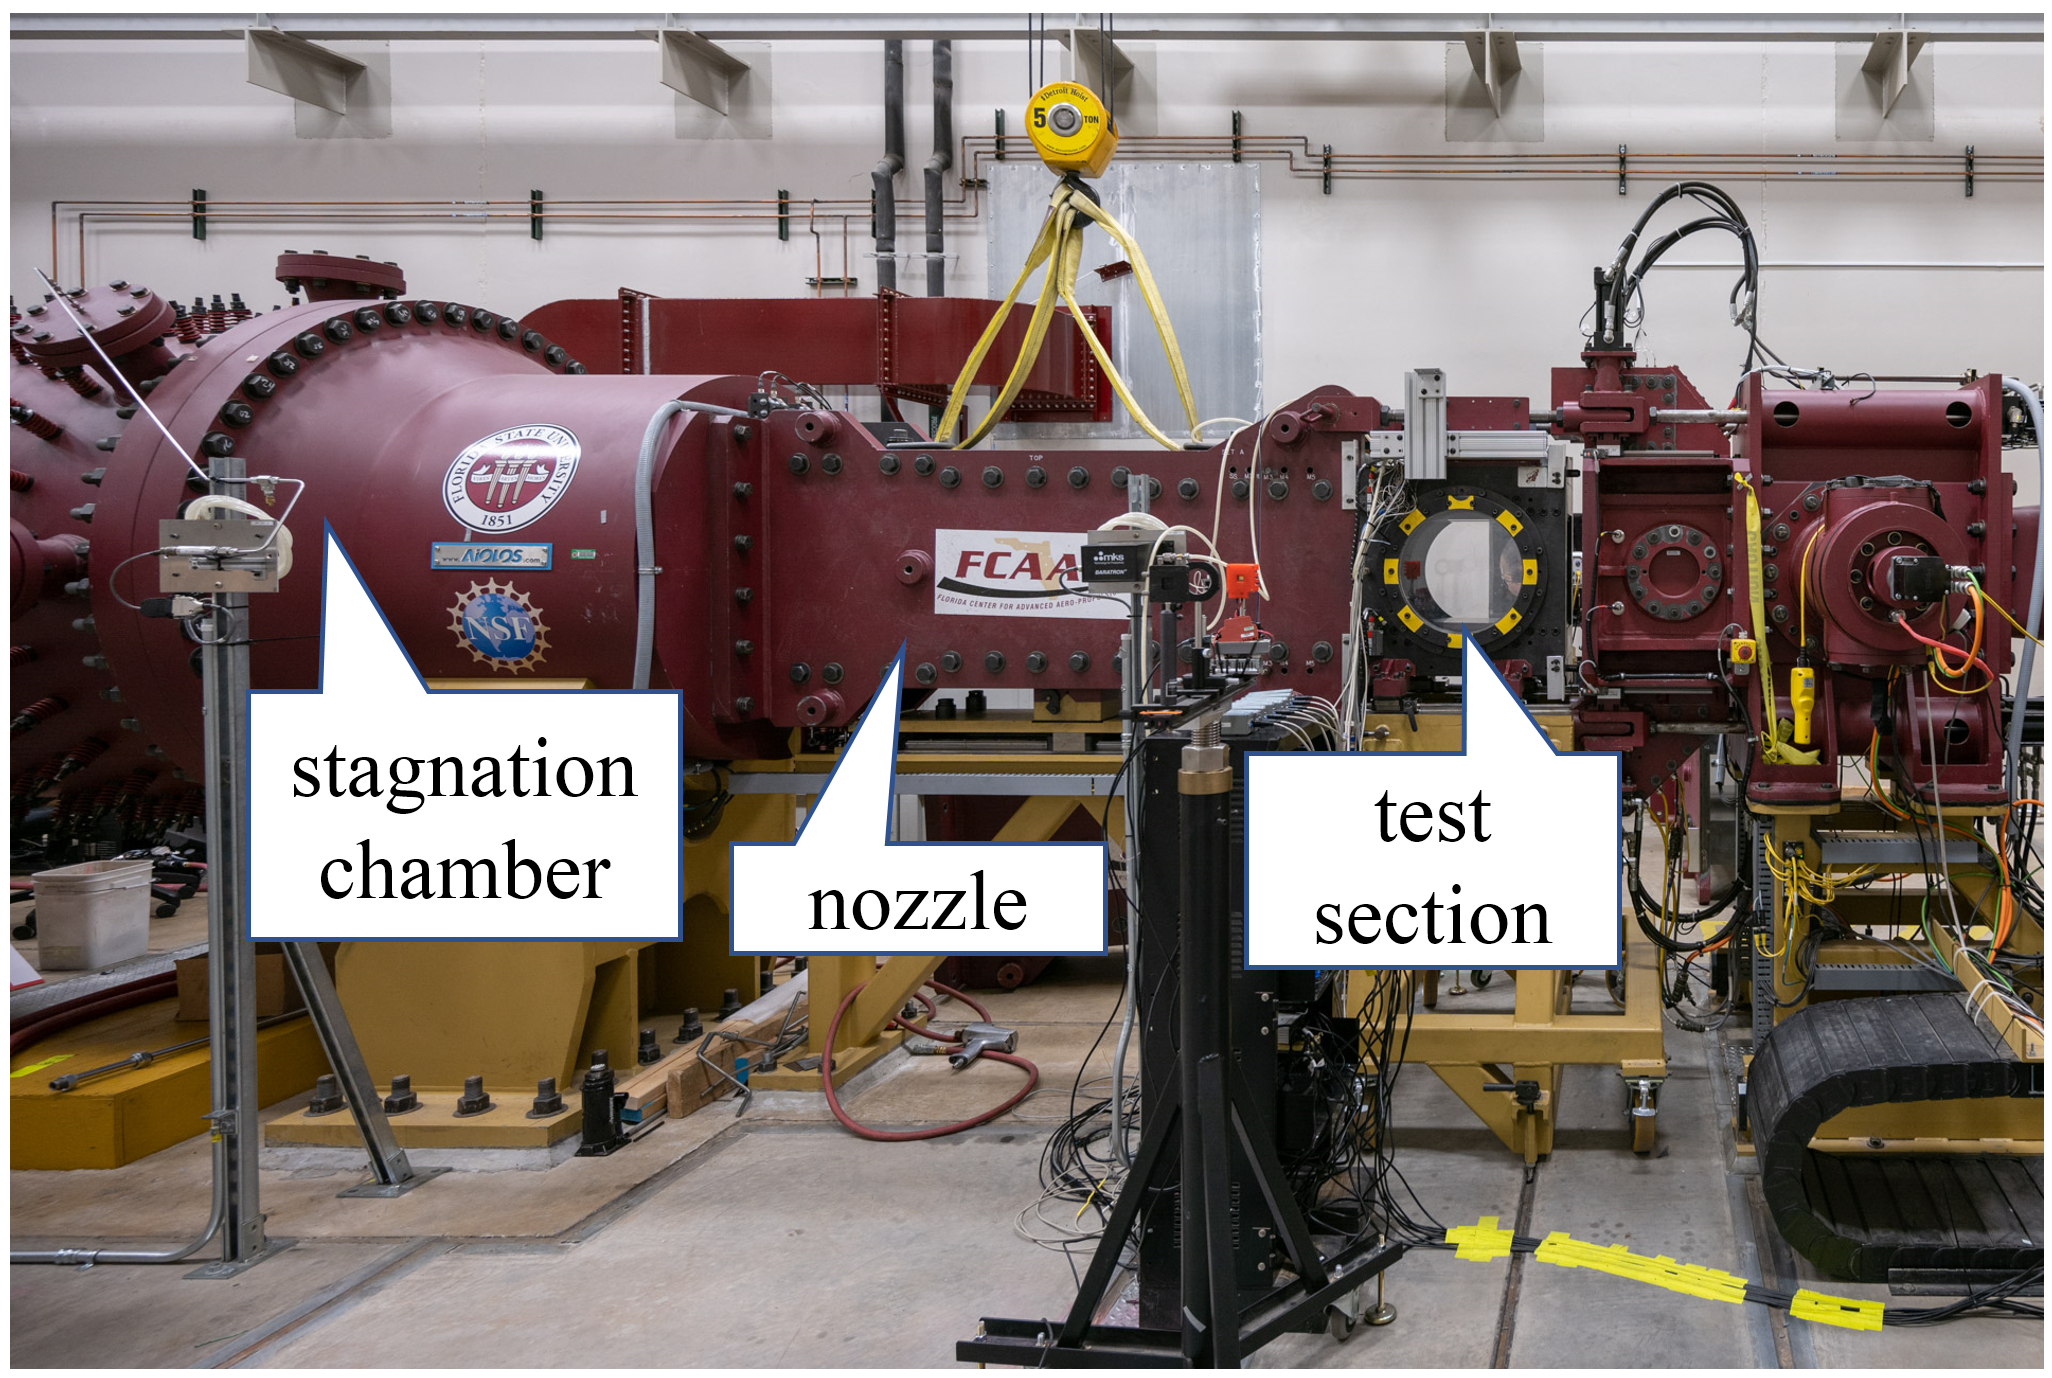
\includegraphics[width=0.7\linewidth]{./figures/fsu/PSWT.PNG}
    \caption{Polysonic wind tunnel}
    \label{fig:PSWT}
\end{figure}

\subsubsection{Test geometry and PIV setup}
The objective of the current set of experiments was to study shock-shock interactions over a range of Mach numbers and shock strengths. For this purpose, a set of wedge shock generators produces leading edge deflections of 5, 10, and $15^\circ$. The shock generators have a spanwise width of 0.14 m, which is a compromise between maintaining 2D flow on the tunnel centerline and keeping flow blockage low. To limit spanwise edge effects, the shock generators are mounted on diamond cross-section struts from the test section ceiling and floor, as shown in \ref{fig:PIVsetup}.\par

A laser sheet was introduced through a window installed in the top test section plug downstream of the top strut to allow PIV measurements in a vertical streamwise plane between the shock generators. The laser used was an Evergreen EVG-200 200mJ per pulse Nd:YAG laser operated at a 7.23 Hz repetition rate and an inter-pulse spacing of 0.8, 1.0, and 0.7 $\mu s$ at Mach 2, 3, and 4, respectively. Planar PIV imaging was carried out through the side window using two Lavision Imager Pro X cameras in parallel to provide two overlapping fields of view adjusted for each Mach number as the region of interest varied. At Mach 2, Camera 1 (wide) used a 50mm lens with a 1.4x teleconverter, and Camera 2 (zoomed in) used a 135mm lens with a 1.4x teleconverter. For Mach 3, the lenses were 135mm and 180mm, respectively, without teleconverters. Finally, at Mach 4, the lenses chosen were 50mm without a teleconverter for Camera 1 and 180 mm lens with a 1.4x teleconverter for Camera 2.\par

\begin{figure}[ht!]
    \centering
    \includegraphics[width=0.7\linewidth]{./figures/fsu/PIVsetup.PNG}
    \caption{Test section side view showing shock generators on struts and the PIV laser sheet optics on top of the test section.}
    \label{fig:PIVsetup}
\end{figure}

\subsubsection{Seeding setup}
For this set of PIV tests, seeding was provided by a Wright nebulizer installed in a flanged pressure vessel as shown in \ref{fig:seedsystem}. Before testing, the pressure vessel was filled above the nebulizer with Rosco Fog Fluid, a commercial fog generator fluid also used in low-pressure, heat-based fog generators. This is a viscous liquid consisting of various glycols in a water solution with a density of 1055-1075 kg/m\textsuperscript{3}. The seeder is provided air from the same high-pressure system as the wind tunnel with a regulator allowing the pressure to be set before the start of each tunnel blowdown and a solenoid valve allowing seeding to be started and stopped remotely from the control room after the tunnel has been started and after the completion of PIV image acquisition, respectively. The pressure must be adjusted to be larger than the stagnation pressure in each run to ensure good seeding. Here, the regulator outlet pressures were set at 0.55, 0.69, and 1.38 MPa for Mach 2, 3, and 4, respectively. At Mach 4, the seeding pressure was limited by the pressure rating of the seeder pressure vessel, and seeding was found to be less dense and consistent compared to the lower Mach numbers. Downstream of the nebulizer, the seed stream is fed into the wind tunnel stagnation chamber downstream of the flow conditioning meshes, but upstream of the convergence, it leads into the nozzle. The tunnel has two flanged ports, one on top and one on bottom, which can be used to install a vertical seeder pipe with an outer diameter of 32 mm and an inner diameter of 27 mm. Two different pipes are available - a half-length that utilizes a single port for seeding close to either the ceiling or the wind tunnel floor or a full length providing seeding in the center of the test section. In this setup, which was used in the present set of tests, five 3.2-mm diameter holes facing upstream in the stagnation chamber are drilled into the vertical seed pipe to deliver the air-seed mixture into the chamber and ensure good mixing before it is convected into the test section. This arrangement, as well as the approximate 6 m of hose connecting the seeder to the seed pipe, likely impacts the delivered seed particle distribution as larger particles will tend to settle on walls and in bends as they are transported by low-velocity air to the stagnation chamber.
% FSU: Please add information about the setup. I can edit as needed. Thanks!

\begin{figure}[ht!]
        \centering
    \begin{subfigure}{0.35\linewidth}
        \centering
        \includegraphics[width=\linewidth]{./figures/fsu/Seeder_a.PNG}
        \caption{Wright nebulizer assembly removed from pressure vessel}
        \label{fig:wrightneb}
    \end{subfigure}%
    \begin{subfigure}{0.35\linewidth}
        \centering
        \includegraphics[width=\linewidth]{./figures/fsu/Seeder_b.PNG}
        \caption{Seeder shown with air supply line and outlet connected to top port on tunnel stagnation chamber}
        \label{fig:seedcon}
    \end{subfigure}
    \caption{Seeding system used for PIV measurements in the Polysonic Wind Tunnel}
    \label{fig:seedsystem}
\end{figure}
\subsubsection{PIV processing}


\subsection{Effect of particle size and density on the response}
The effect of particle size and density on particle response time has been widely studied in an oblique shock problem both experimentally (e.g. Ragni et al. \cite{ragni2011}) and numerically (e.g. Williams et al. \cite{williams2015}). In this section, a similar study was conducted using the current LPT code. These analyses show the current capability of the code and provide an easy-to-use approach for numerical analysis of the oblique shock response. The Loth drag model is considered to track particles unless specified.\par

This section will be added to the final version of the dissertation.\par



% vary mach regimes and conduct the analysis -- williams had done it
\subsection{Benchmarking drag models}
In this section, different drag models implemented in the code are benchmarked for their reliability and performance to use for a response analysis across different Mach regimes.

This section will be added to the final version of the dissertation.\par

% Do the polydisperse analysis for particle distribution variation vs. particle relaxation length observed in experiments
\subsection{Polydisperse analysis - Stochastic model}
Until this point, only the mean particle size and density have been used to perform the particle response analysis. This is done because the underlying distribution of particle size and density is unknown due to agglomeration. In this section, the effect of size variation using multiple distributions is studied to understand the impact on response time. This study is important to The current LPT code has the ability to input a distribution of particles to track them simultaneously in a flow field and obtain their paths.\par

This section will be added to the final version of the dissertation.\par


It is established in several works (Urban and Mungal \cite{urban2001}, Mitchell et al. \cite{mitchell2011}, and Williams et al. \cite{williams2015}) that the particle properties during a PIV run vary in comparison to the distribution obtained from the seeder. This is due to two factors: agglomeration/breakup, which affects the mean particle size and density, and the ability of particles to reflect light that is captured by the camera sensor, which skews the particle distribution observed in the images. These factors make it essential to understand the particle distribution picked up by the PIV imaging system, which can help estimate the range of Stokes number. This helps define uncertainty bounds due to tracer particles in a PIV experiment. The size distribution analysis described in the previous section is extended to the shock interaction PIV experiments in this section.\par

Two different shock interaction cases were studied for the current study. The first case involved a Mach 2.0 flow with shock generators configured at deflection angles of $5^\circ$ and $5^\circ$, while the second configuration utilized deflection angles of $10^\circ$ and $10^\circ$. The corresponding shadowgraphs for these configurations are presented in Fig. \ref{fig:shadowgraph_shock_interaction}, illustrating the resultant shock structures and interaction regions. These visualizations provide critical insights into the flow characteristics, including the shock wave formations, interaction patterns, and potential separation zones.\par

The comparison of these cases underscores the influence of deflection angles on the complexity and intensity of shock interactions. The incident shocks formed from the deflectors are isolated to estimate the particle distribution. This approach minimizes interference from other flow features that happen in the post-interaction region, ensuring a more accurate assessment within the designated region.\par

\begin{figure}[ht!]
    \begin{subfigure}{0.5\linewidth}
        \centering
        \includegraphics[width=\linewidth]{./figures/fsu/Mach2_5_5.png}
        \caption{Mach2 - $5^\circ$ and $5^\circ$}
        \label{fig:shadowgraph_shock_interaction1}
    \end{subfigure}%
    \begin{subfigure}{0.5\linewidth}
        \centering
        \includegraphics[width=\linewidth]{./figures/fsu/Mach2_10_10.png}
        \caption{Mach2 - $10^\circ$ and $10^\circ$}
        \label{fig:shadowgraph_shock_interaction2}
    \end{subfigure}
    \caption{Shadowgraphs of shock interaction cases under study}
    \label{fig:shadowgraph_shock_interaction}
\end{figure}

The data obtained from the PIV experiment is processed using DaVis 11.2 software. The average velocity contours are obtained with multiple interrogation windows with 75\% overlap. This data is normalized using Eq. \ref{eq:exponential_decay}, and the data at each node in the grid is plotted against the x-direction. To establish a consistent reference, the incident shock location was set to zero by identifying the velocity drop characteristic of the shock. The data was further refined to isolate information from the incident shock region. This filtering was achieved by utilizing the post-shock velocity predicted from isentropic oblique shock relations. The resulting data is presented in Fig. \ref{fig:shock_location_plot}. The observed spread in the data is attributed to the particle size and the interrogation window size, which was 64×64 for the current case.\par

\begin{figure}[ht!]
    \begin{subfigure}{0.5\linewidth}
        \centering
        \includegraphics[width=\linewidth]{./figures/fsu/M2_5_5_64x64_normalized.png}
        \caption{Mach2 - $5^\circ$ and $5^\circ$}
        \label{fig:shock_location_plot1}
    \end{subfigure}%
    \begin{subfigure}{0.5\linewidth}
        \centering
        \includegraphics[width=\linewidth]{./figures/fsu/M2_10_10_64x64_normalized.png}
        \caption{Mach2 - $10^\circ$ and $10^\circ$}
        \label{fig:shock_location_plot2}
    \end{subfigure}
    \caption{Shock location adjusted normalized velocity}
    \label{fig:shock_location_plot}
\end{figure}

The data from Fig. \ref{fig:shock_location_plot} is further reduced by removing any velocity below the post-shock velocity. This helps isolate the data relevant to the oblique shock. An uncertainty bound of 0.5\% was incorporated during this data reduction process to account for uncertainties inherent in the image analysis. For instance, in the case of a Mach 2.0 flow with a deflection angle of $5^\circ$, the pre-shock velocity was set to $510m/s$, and the post-shock velocity was determined to be $480m/s$. This approach ensures a robust analysis of the shock region while mitigating the impact of measurement uncertainties.\par

The nominal diameter and density of the particle were computed using the two-equation approach presented in section \ref{sec:lpt}. The diameter and density of the particles were estimated to be $0.808 \mu m$ and $1408 kg/m^3$, respectively.\par

Understanding that the current particle sizing analysis depends on the uncertainties arising throughout the PIV experiment is essential. Lazar et al. \cite{lazar2010} showed that most uncertainty arises from particle dynamics and cross-correlation performed in PIV for a supersonic crossflow case. Since isolating the uncertainty generated from the analysis aspect is currently not possible, a sensitivity analysis is performed to understand the particle size distribution. The methodology described in the previous section is applied to the isolated data present in Fig. \ref{fig:shock_location_plot}.\par

% TODO: We might need to add the two-equation two-variable (diameter and density) problem.

% 
\subsection{Mach 2.0 $5^\circ/5^\circ$}
The results obtained for different interrogation window sizes for Mach 2.0 $5^\circ/5^\circ$ case are presented in Fig. \ref{fig:dia_distribution_5-5}. The histograms in each subplot represent the distribution of particle diameters in microns under different spatial resolutions. These distributions are multimodal, indicating the presence of distinct particle groups being detected during the experiment. This can happen for several reasons, such as agglomeration, breakup, or heterogeneous particle generation. The spatial resolution significantly influences the density peaks and smoothness of the distributions. For example, the highest resolution case (0.087 mm) captures finer details of the size distribution, showing sharper and more frequent peaks compared to the coarsest (0.465 mm) resolution case, which could suggest a loss of information relevant to particle sizes resulting from the analysis. This implies that the larger particles dominate the signal strength in coarser resolutions, and broader distributions average out the particle characteristics.\par

\begin{figure}[ht!]
    \centering
    \includegraphics[width=\linewidth]{figures/fsu/diameter_distribution_5-5.png}
    \caption{Particle diameter distributions for Mach 2.0 $5^\circ/5^\circ$ case at different spatial resolutions}
    \label{fig:dia_distribution_5-5}
\end{figure}

The particle size analysis from the PIV data reveals that the mean particle size remains consistent across all spatial resolutions, ranging between $0.8 - 1.0 \mu m$. At finer spatial resolutions (e.g., 0.087 mm), the particle size distribution appears almost uniform, showcasing the ability of the PIV system to resolve particles more accurately. This uniformity is crucial for PIV cross-correlation algorithms, as it ensures a balanced contribution from all particle sizes, leading to more reliable and accurate velocity field estimations. In contrast, coarser spatial resolutions (e.g., 0.465 mm) exhibit skewed distributions, with larger particles dominating due to reduced detection of smaller particles. This skewness can introduce biases in velocity estimations, particularly in regions of high gradients, such as oblique shocks, where particle inertia effects are significant. These findings highlight the importance of finer spatial resolutions in preserving the uniform distribution necessary for optimal algorithm performance.\par

% Particle relaxation times and stokes number
% -- Multimodal; Stokes number can be computed using the smallest time scale measurement possible

% flow characteristic time is spatial resolution / max. velocity

\begin{figure}[ht!]
    \centering
    \includegraphics[width=\linewidth]{figures/fsu/stokes_number_distribution_5-5.png}
    \caption{Stokes number distributions for Mach 2.0 $5^\circ/5^\circ$ case at different spatial resolutions}
    \label{fig:stokes_distribution_5-5}
\end{figure}

The Stokes number (St) distributions are analyzed to quantify uncertainties and establish reliable bounds for the measurement setup. The flow characteristic time is determined using the spatial resolution for each case, representing the smallest resolvable size of flow features given a shock wave. While the minimum resolvable size is often chosen based on the specific flow feature under study, spatial resolution frequently imposes a bottleneck.\par

As shown in Figure \ref{fig:stokes_distribution_5-5}, the Stokes number remains below 0.05 for all cases, in accordance with the recommendations of Samimy and Lele (1991). This indicates that the particles closely follow the flow dynamics within acceptable limits of particle inertia effects. However, advancements in interrogation methods, particularly deep learning-based flow reconstruction at the pixel level as reviewed by Yu et al. \cite{yu2023}, are expected to increase the Stokes number if spatial resolution is used as the basis. This suggests that the selection of the flow characteristic time must account for the scale of flow features of interest. This can depend on the turbulence statistics of interest as well. Specifically, in cases involving shock waves, where accuracy is paramount, the flow characteristic time should be computed based on the smallest resolvable scale to ensure precise shock wave representation.

Fig. \ref{fig:stokes_distribution_5-5} further reveals the notable trends in Stokes number distributions across spatial resolutions. Specifically, as spatial resolution coarsens, the mean Stokes number decreases from 0.027 at 0.087 mm resolution to 0.007 at 0.465 mm. This trend reflects reduced particle inertia effects at coarser resolutions, enabling better responsiveness to flow features due to the grid restrictions.\par

The adherence to St < 0.05 across all cases validates the robustness of the setup within the recommended bounds. Spatial resolution directly impacts uncertainty quantification, with higher resolutions providing enhanced certainty in capturing small-scale flow features. For applications involving critical flow features, such as shocks or vortices, the choice of resolution must balance the computational cost and the need for accuracy.\par

% \begin{figure}[ht!]
%     \centering
%     \includegraphics[width=\linewidth]{figures/fsu/response_time_distribution_5-5.png}
%     \caption{Particle response distributions for Mach 2.0 $5^\circ/5^\circ$ case at different spatial resolutions}
%     \label{fig:relaxation_time_5-5}
% \end{figure}


% Finally, the laser pulse time is about $0.8 \mu s$. This is well below the range of relaxation time observed for particles. This is shown in Fig. \ref{fig:relaxation_time_5-5}.

\subsection{Mach 2.0 $10^\circ/10^\circ$}
The results obtained for different interrogation window sizes for the Mach 2.0 $10^\circ/10^\circ$ case are presented in Fig. \ref{fig:dia_distribution_10-10}. The histograms in each subplot represent the distribution of particle diameters in microns under different spatial resolutions. Similar to the $5^\circ/5^\circ$ case, these distributions are multimodal, indicating distinct particle groups detected during the experiment. However, the multimodality is more pronounced for this case and can be distinctly identified for the first three fine resolutions. This indicates that the particles are forming group clusters that are being detected in the images.\par

\begin{figure}[ht!]
    \centering
    \includegraphics[width=\linewidth]{figures/fsu/diameter_distribution_10-10.png}
    \caption{Particle diameter distributions for Mach 2.0 $10^\circ/10^\circ$ case at different spatial resolutions}
    \label{fig:dia_distribution_10-10}
\end{figure}

Like the $5^\circ/5^\circ$ case, the Stokes number, shown in Fig. \ref{fig:stokes_distribution_10-10}, remains well below the recommended threshold for studying supersonic flows. While a stronger shock and larger mean particle diameter would typically result in a higher Stokes number, the distribution in this case exhibits significant right skewness, leading to a Stokes number that is comparable to the $5^\circ/5^\circ$ case. This behavior may be attributed to the breakup of liquid particles as they traverse the shock interface, resulting in smaller particle sizes that reduce the effective Stokes number. It is worth noting that this study does not account for particle agglomeration or breakup dynamics, which may play a significant role in the observed Stokes number distribution under such conditions.\par

\begin{figure}[ht!]
    \centering
    \includegraphics[width=\linewidth]{figures/fsu/stokes_number_distribution_10-10.png}
    \caption{Stokes number distributions for Mach 2.0 $10^\circ/10^\circ$ case at different spatial resolutions}
    \label{fig:stokes_distribution_10-10}
\end{figure}

These results highlight the critical role of spatial resolution and interrogation window size in accurately resolving particle dynamics. For high-gradient flows, such as those involving shocks, finer resolutions are essential to mitigate biases introduced by particle inertia and ensure reliable velocity measurements.\par

\end{comment}

\section{Transformation from Lagrangian to Eulerian data}
The data obtained from the LPT code are in a Lagrangian frame or a scattered format. This data had to be in continuous format to generate PDH-informed synthetic images similar to those obtained from PIV. This was obtained by interpolating the Lagrangian field onto the original oblique shock grid. The transformation process is illustrated in Fig. \ref{fig:oblique_workflow}. The figure illustrates the creation of particle paths from the UC-LPT code and the transformation process to obtain a PDH-informed Eulerian field.\par

\begin{figure}[ht!]
    \centering
    \includegraphics[width=\linewidth]{./figures/03lpt/workflow_contours.png}
    \caption{Workflow to generate PDH-informed Eulerian field from the CFD or analytical data. Top left: Analytical oblique shock solution in the transformed grid; Top right: Particle paths from the UC-LPT code projected onto the same grid; Bottom left: Eulerian field for flow velocity generated from the particle data; Bottom right: Eulerian field for flow velocity generated from the particle data.}
    \label{fig:oblique_workflow}
\end{figure}

Let $\{(x_i, \phi_i)\}_{i=1}^{N}$ be the Lagrangian data points, where:\\
$x_i$ is the position of $i$-th data point in the Lagrangian frame, $\phi_i$ is the scalar (or vector) field value at $x_i$, N is the total number of Lagrangian data points.\\

Let the Eulerian grid be regular and represented as $\{ \textbf{X}_{j}\}_{j=1}^{M}$, where, $\textbf{X}_j$ is the co-ordinates of $j$-th grid point, $M$ is the total number of grid points.

The Lagrangian data is sampled at two data points per cell to capture changes in flow features between cells. This can be represented by $(x_{i_1}, \phi_{i_1})$ and $(x_{i_2}, \phi_{i_2})$. The entire set of sampled data is given by:

\begin{equation}
    \mathcal{L} = \{(x_{i_1}, \phi_{i_1}), (x_{i_2}, \phi_{i_2}) | i = 1, 2, ..., M\}
    \label{eq:lagrangian_sample_set}
\end{equation}

The data on the regular grid is obtained using Scipy's \cite{scipy2020} griddata method, which uses Delaunay triangulation to form a grid from Lagrangian data, and then interpolation is performed onto the regular grid.\par

The Delaunay triangulation is employed here to achieve computational efficiency and ensure a smooth transition between irregularly spaced data, which is necessary due to the implementation of the adaptive particle tracking algorithm. The sampling method, which involves two data points per cell, also facilitates a smooth transition in the data. In tests, especially around shock interfaces, if the sampling algorithm does uniform sampling instead of the current method, inconsistency in data reconstruction was observed.\par

A comprehensive review of the Delaunay triangulation is provided by Elshakhs et al. \cite{delaunay2024}. For a set of points $\mathcal{P}$ in Euclidean space, a triangulation $\mathcal{T}(\mathcal{P})$ is a partitioning of the points into simplices such that no two simplices overlap and every point in the set is a vertex of at least one simplex. For Delaunay triangulation $\mathcal{D}\mathcal{T}(\mathcal{P})$, an additional condition is applied such that no point in $\mathcal{P}$ is inside the circumcircle of any simplex in $\mathcal{D}\mathcal{T}(\mathcal{P})$. This can be understood from Fig. \ref{fig:l2e_delaunay}, where sample data points are randomly distributed. The simplex is constructed using the Delaunay triangulation, and then the data is interpolated onto the regular grid using the weighted averages of simplex vertices.\par

\begin{figure}
    \centering
    \includegraphics[width=\linewidth]{phd_dissertation/figures/03lpt/l2e_transforamtion/delaunay_triangulation.png}
    \caption{Lagrangian to Eulerian format interpolation using Delaunay triangulation}
    \label{fig:l2e_delaunay}
\end{figure}

The weighted interpolation for each Eulerian grid point $\textbf{X}_j$ is given by Eq. \ref{eq:l2e_interpolation}.\par

\begin{equation}
    \Psi(\textbf{X}_j) = \sum_{m=1}^3 \mathcal{W}(\textbf{X}_{i_m})\phi_{i_m}
    \label{eq:l2e_interpolation}
\end{equation}

where, $\mathcal{W}(\textbf{X}_{i_m})$ is determined based on the distance of grid node $\textbf{X}_j$ from the simplex vertices obtained from $\mathcal{D}\mathcal{T}(\mathcal{P})$.

For the current analysis, monodisperse particles were used to quantify the error introduced by interpolating to the Eulerian frame. The data obtained from the LPT code were converted to an Eulerian frame by linear interpolation. The UC-LPT code has the framework to produce data in a structured plot3D format, as presented by Walatka et al. \cite{walatka1990}. Fluid data was also collected at these scattered points and fitted to capture any uncertainty arising from the conversion process. This maintains consistency; typically, this uncertainty cancels out when comparing data for particle inertia bias. The Eulerian frame data for the shock-normal velocity are presented in Fig. \ref{fig:oblique_workflow} for interpolated particle and fluid fields. It can be observed from the figure that the availability of data corresponds to the regions of particle presence in the flow field. The rest of the flow field has an outlier value, making differentiating regions without the particle field easy.\par

A grid convergence analysis where the interpolation is tested on several grid sizes yielded no difference in the interpolated data, showcasing the superiority of the current method.\par

\begin{comment}
Due to the nature of the sampling implemented, there might be regions of error depending on the grid size. These usually happen when there is a sudden change in the data, such as shocks in the current case. This can be rectified using larger data sets and finer grids for the interpolation, which is possible with better hardware to run the program. In the current case, a convergence analysis is performed based on four different grid sizes, and the results are presented in Fig. \ref{fig:compare_dataio_to_paths}. For the rest of the analysis, the finest grid size tested was used. The maximum error for the 2000x2000 grid occurs at the shock interface and is calculated to be 0.04\%. The average error is negligible. This indicates that the data has been transformed from the Lagrangian frame to the Eulerian frame without any numerical error due to interpolation.\par

\begin{figure}[ht!]
    \centering
    \includesvg[width=0.7\linewidth]{./figures/03lpt/compare_dataio_to_paths_gca}
    \caption{Grid convergence analysis for Lagrangian to Eulerian transformation}
    \label{fig:compare_dataio_to_paths}
\end{figure}
\end{comment}


% Grid convergence study
% Data convergence study
% Nearest vs. Linear vs. Quadratic vs. Cubic

\section{Notes on Parallelization}
The particle tracking and data conversion methods described in this chapter utilize parallelization through the Message Passing Interface (MPI) library, implemented in Python. This approach distributes the computational workload across multiple processors, significantly enhancing efficiency.\par

The motion of each particle and related computations are processed independently, making them ideal for parallelization. MPI assigns the calculation of an individual or a group of particles to different processors. This ensures that all particles are tracked simultaneously across the domain by reducing the CPU wall clock time.\par

The process of converting the data involves mapping particle information onto a grid. This parallelization is achieved by dividing the grid into smaller subdomains, with each subdomain assigned to a processor. Then, MPI scatters the data, distributing these subdomains to different processors for independent processing. Once the interpolation is done, MPI gathers these results, and the data from subdomains are combined to form the complete domain.\par

This parallelization approach ensures that particle tracking and data conversion are efficient and scalable. The code can be easily deployed to both personal and high-performance computing (HPC) using the PyPI repository.\par

\section{Summary}
This chapter details the development, implementation, and application of Lagrangian Particle Tracking (LPT) for supersonic flow studies. Each aspect of the LPT has been meticulously modeled and enhanced using existing algorithms, with new approaches introduced to improve accuracy and efficiency. For instance, the time taken for the p-space search algorithm has been significantly reduced (approximately 32 times faster) by providing an improved initial guess for the Newton-Raphson method, as demonstrated in a test case with 42 million nodes. Various interpolation techniques, including radial basis functions (RBF), shock cell interpolation, and linear methods, have been implemented and analyzed for speed and accuracy. While RBF interpolation proved computationally intensive, it provided accurate approximations on coarser grids. A novel shock cell interpolation method ensured accuracy in shock regions where linear methods faltered. Additionally, the stability of multiple Runge-Kutta integration methods was assessed using a hypothetical vortex test case, contributing to a more robust implementation.

\begin{comment}
The chapter emphasizes the importance of particle size distribution analysis in understanding particle response times under oblique shock conditions. Using Gaussian and skew-normal distributions, the analysis reveals how variations in particle diameters, influenced by agglomeration or breakup, affect response times and flow diagnostics. A novel methodology combining z-statistics, curve fitting, and response time distributions was introduced, enabling accurate predictions of underlying particle distributions. The results indicate that accounting for polydispersity in particles is critical for minimizing uncertainty in particle image velocimetry (PIV) measurements, particularly in high-variance scenarios.

The experimental analysis included two oblique shock cases at Mach 2.0 with $5^\circ/5^\circ$ and $10^\circ/10^\circ$ deflection angles, highlighting the role of spatial resolution and interrogation window size on particle dynamics. Finer spatial resolutions ensured better uniformity in particle size distributions and accurate representation of high-gradient flow features like shocks, while coarser resolutions introduced biases. Stokes number analysis confirmed adherence to established thresholds (St < 0.05), validating the robustness of the methodology while underscoring the need to account for spatial resolution and flow characteristics in future studies.
\end{comment}

A key contribution of the chapter is transforming Lagrangian particle data into an Eulerian frame, which simplifies the data. This process was implemented using Delaunay triangulation and adaptive sampling to ensure smooth data transitions, particularly in shock regions. The methodology was validated through grid convergence studies, which confirmed negligible interpolation errors, even in high-gradient zones. The resulting Eulerian data preserves particle dynamics history (PDH) and provides a foundation for understanding uncertainties related to particle presence and behavior in flow diagnostics.

Parallelization techniques were employed to enhance computational efficiency, leveraging the Message Passing Interface (MPI). By distributing workload across processors for particle tracking and interpolation, the code demonstrated scalability for large-scale simulations, with direct applicability to high-performance computing (HPC) environments.

Furthermore, the LPT code integrates advanced drag models, such as the Loth drag model, which effectively accounts for compressibility and rarefaction effects. Validation against oblique shock response tests demonstrated the model's capability to accurately capture particle dynamics, reaffirming the importance of considering particle agglomeration and breakup in response time analyses. Comparisons with experimental results, such as those by Williams et al. \cite{williams2015}, highlighted the accuracy and reliability of the implemented methodologies.

In summary, the chapter presents a comprehensive framework for Lagrangian Particle Tracking, encompassing advanced algorithmic enhancements, robust drag modeling, accurate particle size distribution analysis, and efficient parallelization. These contributions significantly advance the understanding of particle dynamics in supersonic flows, offering a robust toolset for PIV studies and other high-speed flow diagnostics. The methodologies presented improve experimental accuracy and lay the groundwork for future research in supersonic and multiphase flow analysis.